\documentclass{ximera}

\begin{document}
	\author{Stitz-Zeager}
	\xmtitle{TITLE}


\mfpicnumber{1}

\opengraphsfile{LogarithmicEquationsandInequalities}

\setcounter{footnote}{0}

\label{LogarithmicEquationsandInequalities}

In Section \ref{ExponentialEquationsandInequalities} we solved equations and inequalities involving exponential functions using one of two basic strategies.  We now turn our attention to equations and inequalities involving logarithmic functions, and not surprisingly, there are two basic strategies to choose from.  

\smallskip

For example, per Theorem \ref{explogsonetoone}, the \textit{only} solution to $\log_{2}(x) = \log_{2}(5)$ is $x=5$.   Now consider $\log_{2}(x) = 3$.  To use Theorem \ref{explogsonetoone}, we need to rewrite $3$ as a logarithm base $2$.   Theorem \ref{invpropslogs} gives us $3 = \log_{2}\left(2^{3}\right) = \log_{2}(8)$.  Hence, $\log_{2}(x) = 3$ is equivalent to  $\log_{2}(x) =  \log_{2}(8)$ so that $x = 8$. 

\smallskip

A second approach to solving  $\log_{2}(x) = 3$ us to apply the corresponding exponential function, $f(x) = 2^x$ to both sides:  $2^{\log_{2}(x)} = 2^{3}$ so $x = 2^3 = 8$.

\smallskip

A third approach to solving  $\log_{2}(x) = 3$ is to use  Theorem \ref{invpropslogs} to rewrite $\log_{2}(x) = 3$ as $2^{3} = x$, so  $x=8$.   

\smallskip

In the grand scheme of things, all three approaches we have presented to solve $\log_{2}(x) = 3$ are mathematically equivalent, so we opt to choose the last approach in our summary below.

\smallskip

\colorbox{ResultColor}{\bbm

\centerline{\textbf{Steps for Solving an Equation involving Logarithmic Functions}} \index{logarithm ! solving equations with} 

\begin{enumerate}

\item  Isolate the logarithmic function.

\item  \begin{enumerate}

\item  If convenient, express both sides as logs with the same base and equate arguments.

\item  Otherwise, rewrite the log equation as an exponential equation.


\end{enumerate}

\end{enumerate}

\smallskip

\ebm}

\smallskip

\begin{example}  \label{LogEqnsEx1} Solve the following equations.  Check your solutions graphically using a calculator.

\begin{multicols}{2}
\begin{enumerate}

\item  $\log_{117}(1-3x) = \log_{117}\left(x^2-3\right)$

\item  $2 - \ln(t-3) = 1$

\setcounter{HW}{\value{enumi}}
\end{enumerate}
\end{multicols}

\begin{multicols}{2}
\begin{enumerate}
\setcounter{enumi}{\value{HW}}

\item  $\log_{6}(x+4) + \log_{6}(3-x) = 1$

\item  $\log_{7}(1-2t) = 1 - \log_{7}(3-t)$
\setcounter{HW}{\value{enumi}}
\end{enumerate}
\end{multicols}

\begin{multicols}{2}
\begin{enumerate}
\setcounter{enumi}{\value{HW}}

\item  $\log_{2}(x+3) = \log_{2}(6-x)+3$

\item  $1 + 2 \log_{4}(t+1) = 2 \log_{2}(t)$

\end{enumerate}
\end{multicols}

{\bf Solution.}

\begin{enumerate}

\item  Since we have the same base on both sides of the equation $\log_{117}(1-3x) = \log_{117}\left(x^2-3\right)$, we equate the arguments (what's inside) of the logs to get $1-3x = x^2-3$.  Solving $x^2+3x-4 = 0$ gives $x=-4$ and $x=1$. 

\smallskip

To check these answers using a graphing utility,  we make use of the change of base formula and graph $f(x) = \frac{\ln(1-3x)}{\ln(117)}$ and $g(x) = \frac{\ln\left(x^2-3\right)}{\ln(117)}$.  We see these graphs intersect only at $x=-4$. however.  

\smallskip

To see what happened to the solution $x=1$, we substitute it into our original equation to obtain  $\log_{117}(-2) =  \log_{117}(-2)$.  While these expressions look identical, neither is a real number,\footnote{They do, however, represent the same \textbf{family} of complex numbers.  We refer the reader to a course in Complex Variables.} which means $x=1$ is not in the domain of the original equation, and is not a solution.    


\item  To solve  $2 - \ln(t-3) = 1$, we first isolate the logarithm and get $\ln(t-3) = 1$. Rewriting $\ln(t-3) = 1$ as an exponential equation, we get is $e^{1} = t-3$, so $t =e+3$. 

\smallskip

A graphing utility shows the graphs of $f(t) = 2 - \ln(t-3)$ and $g(t) = 1$ intersect at $t \approx   5.718 \approx e+3$.

\begin{center}

\begin{tabular}{cc}

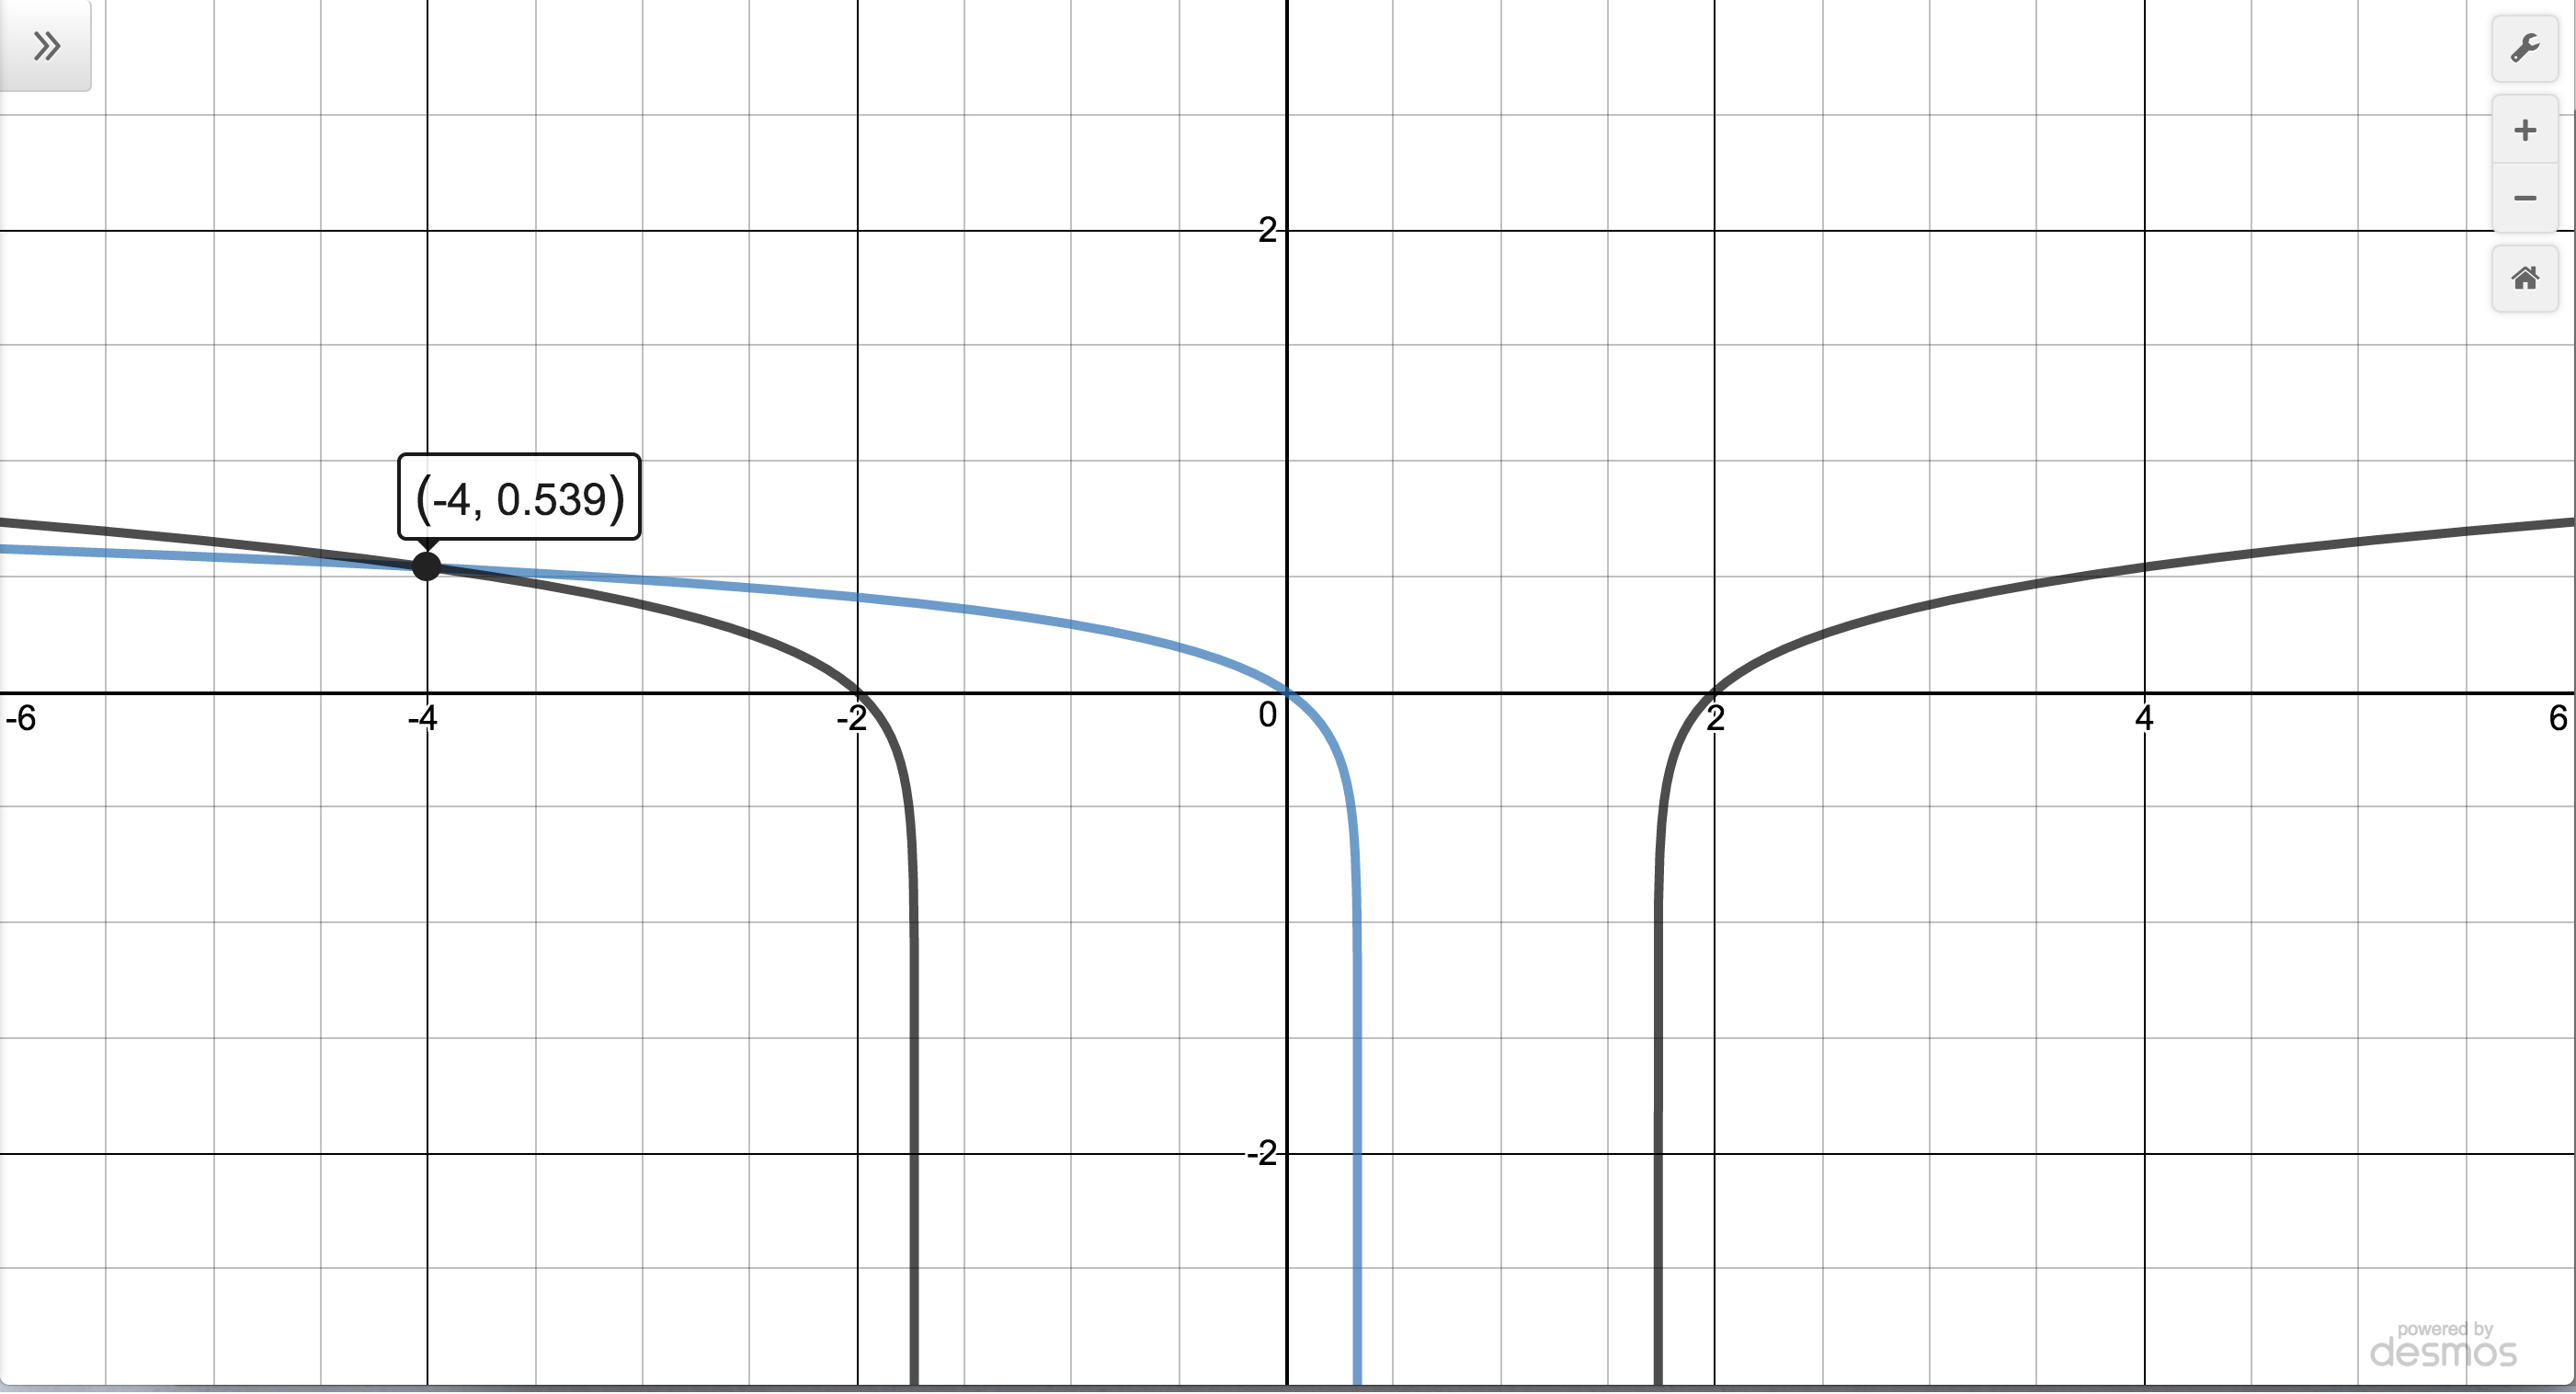
\includegraphics[width=3in]{./LogarithmicEquationsandInequalitiesGraphics/LogEqnEx01.jpg} &

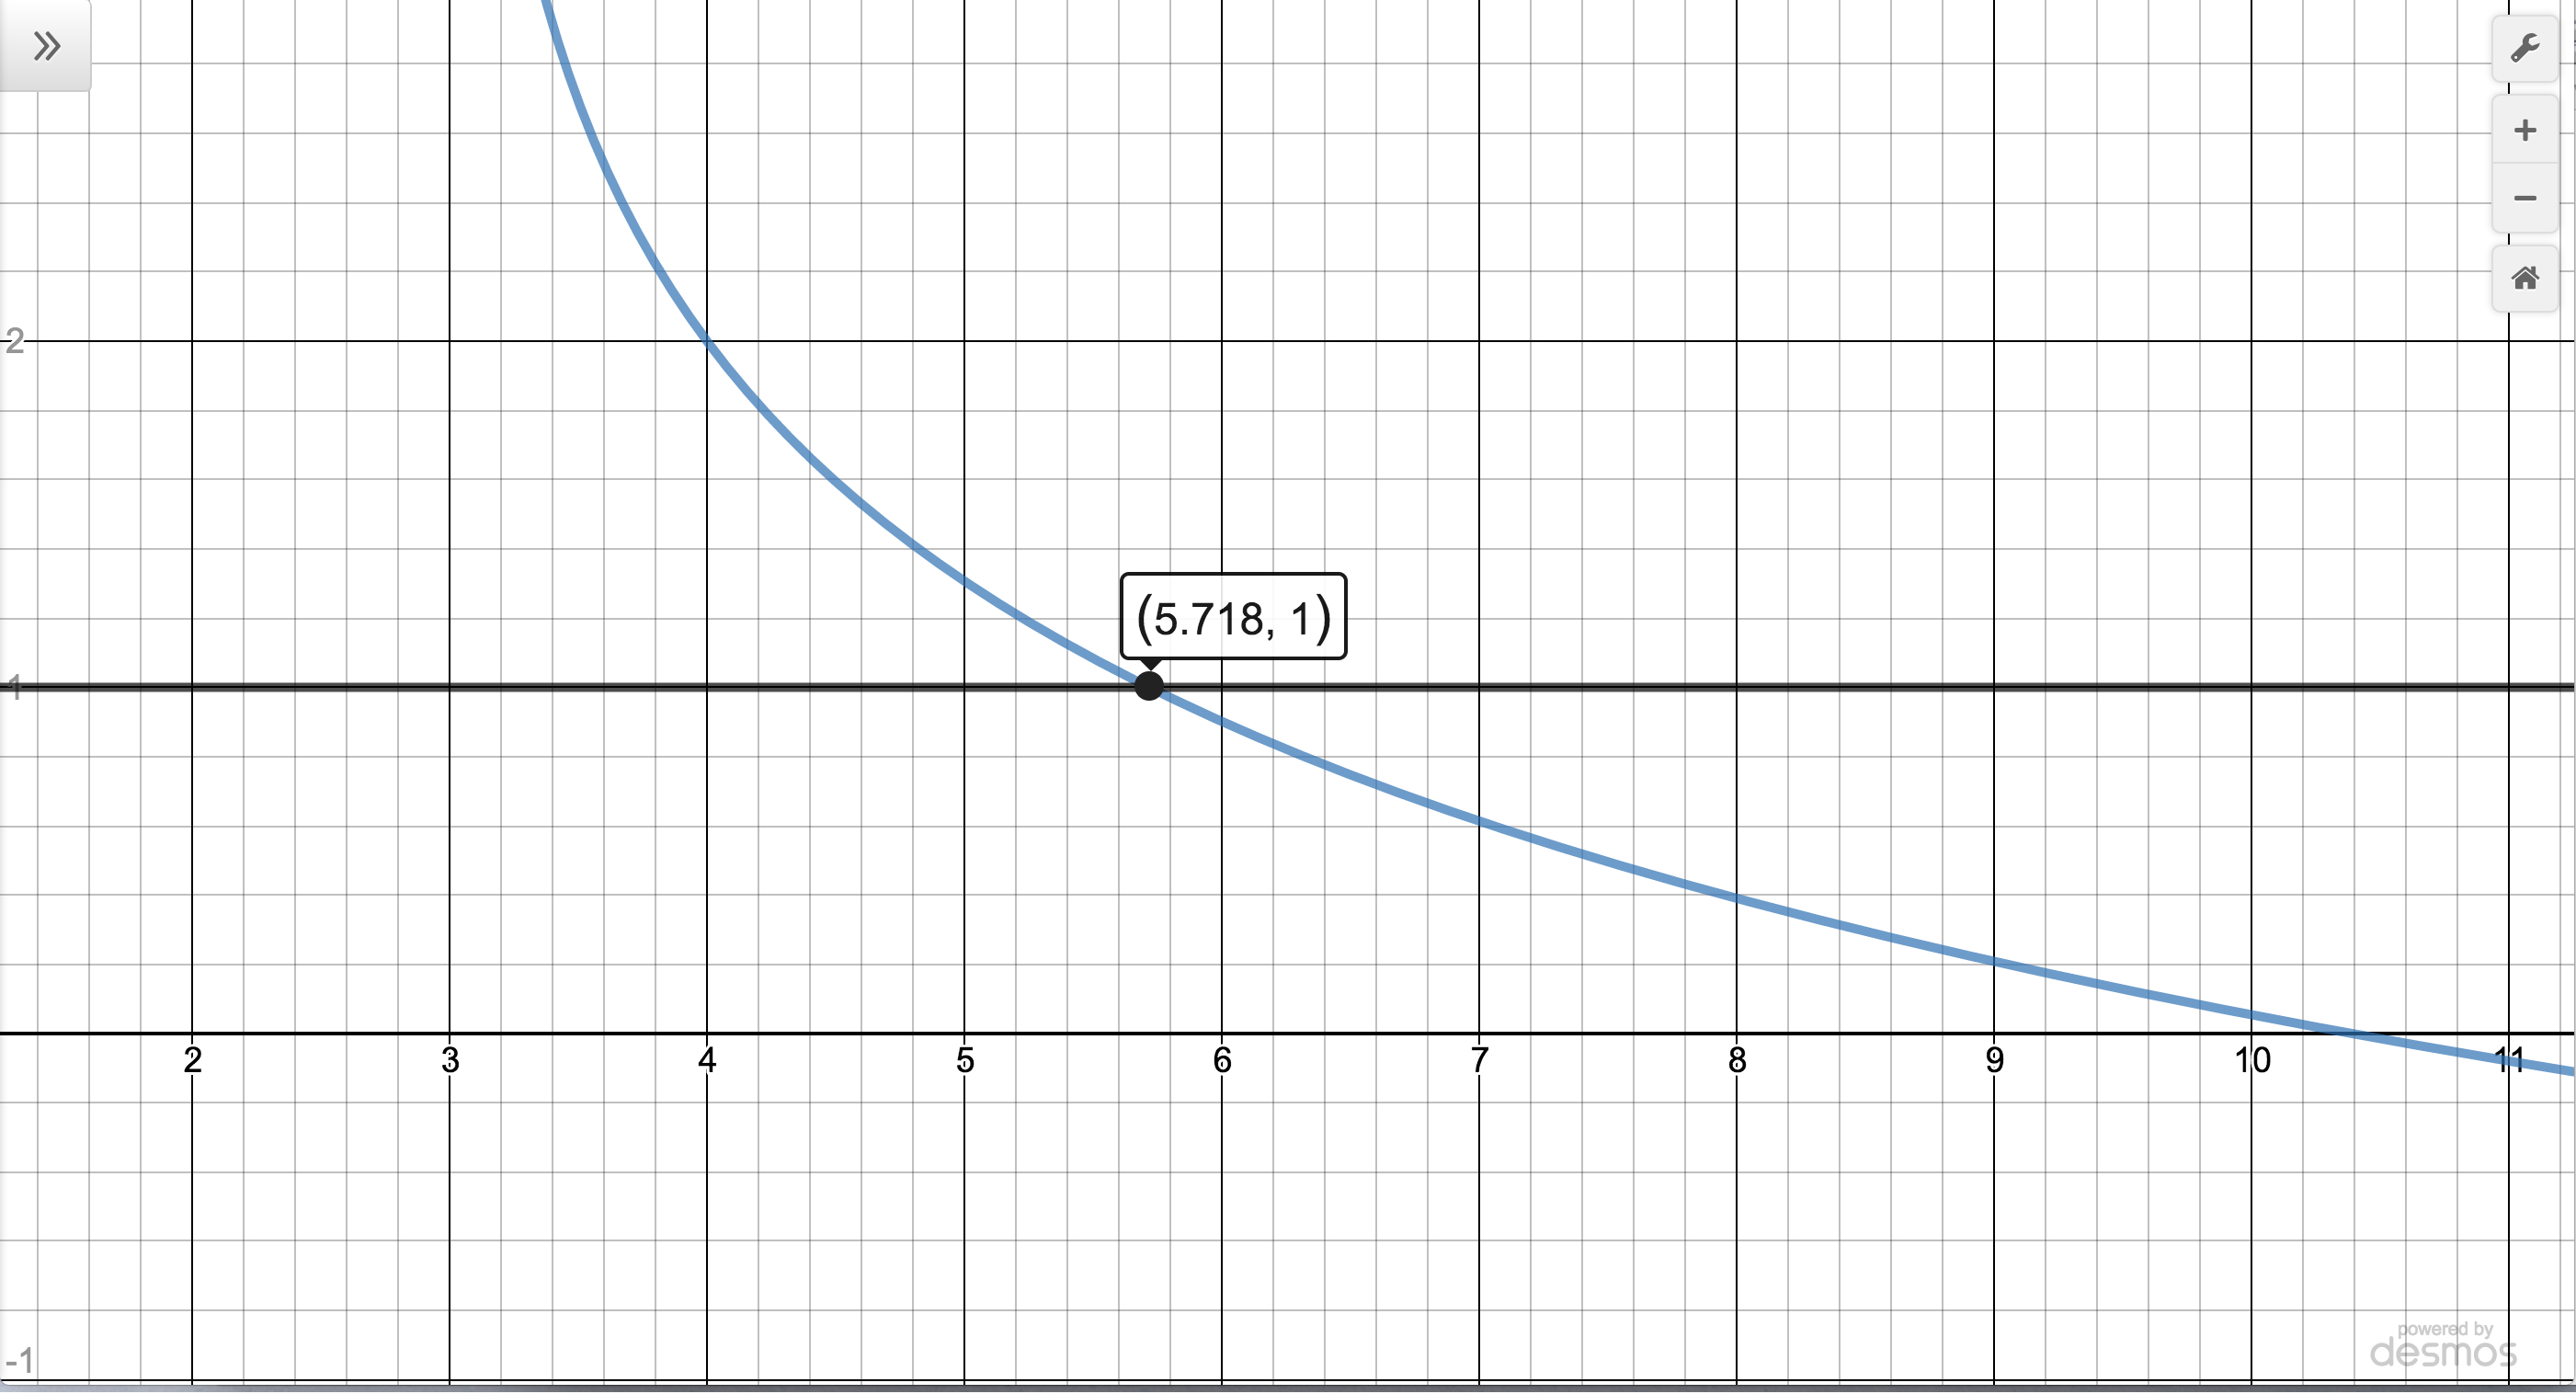
\includegraphics[width=3in]{./LogarithmicEquationsandInequalitiesGraphics/LogEqnEx02.jpg}  \\

Checking $\log_{117}(1-3x) = \log_{117}\left(x^2-3\right)$
 
 &
 
 Checking $2 - \ln(t-3) = 1$
 
\end{tabular}

\end{center}


\item We  start solving $\log_{6}(x+4) + \log_{6}(3-x) = 1$ by using the Product Rule for logarithms to rewrite the equation as  $\log_{6}\left[(x+4)(3-x)\right] = 1$.  

\smallskip

Rewriting as an exponential equation gives $6^{1} = (x+4)(3-x)$ which reduces to $x^2+x-6 = 0$.  We get two solutions: $x=-3$ and $x=2$.   

\smallskip

Using the change of base formula, we graph  $y=f(x) =  \frac{\ln(x+4)}{\ln(6)} + \frac{\ln(3-x)}{\ln(6)}$ and $y=g(x) = 1$ and we see the graphs intersect twice, at $x=-3$ and $x=2$, as required.

\item  Taking a cue from the previous problem, we begin solving $\log_{7}(1-2t) = 1 - \log_{7}(3-t)$ by first collecting the logarithms on the same side, $\log_{7}(1-2t) +  \log_{7}(3-t) = 1$, and then using the Product Rule to get $\log_{7}[(1-2t)(3-t)] = 1$.  

\smallskip

Rewriting  as an exponential equation gives $7^{1} = (1-2t)(3-t)$ which gives the quadratic equation $2t^2-7t-4=0$.  Solving, we find  $t = -\frac{1}{2}$ and $t=4$.  

\smallskip

Once again, we use the change of base formula and find the graphs of  $y = f(t) = \frac{\ln(1-2t)}{\ln(7)}$ and $y=g(t) = 1 - \frac{\ln(3-t)}{\ln(7)}$ intersect only at $t=-\frac{1}{2}$.  

\smallskip

Checking $t=4$ in the original equation produces $\log_{7}(-7) = 1 - \log_{7}(-1)$, showing $t=4$ is not in the domain of $f$ nor $g$.

\begin{center}

\begin{tabular}{cc}

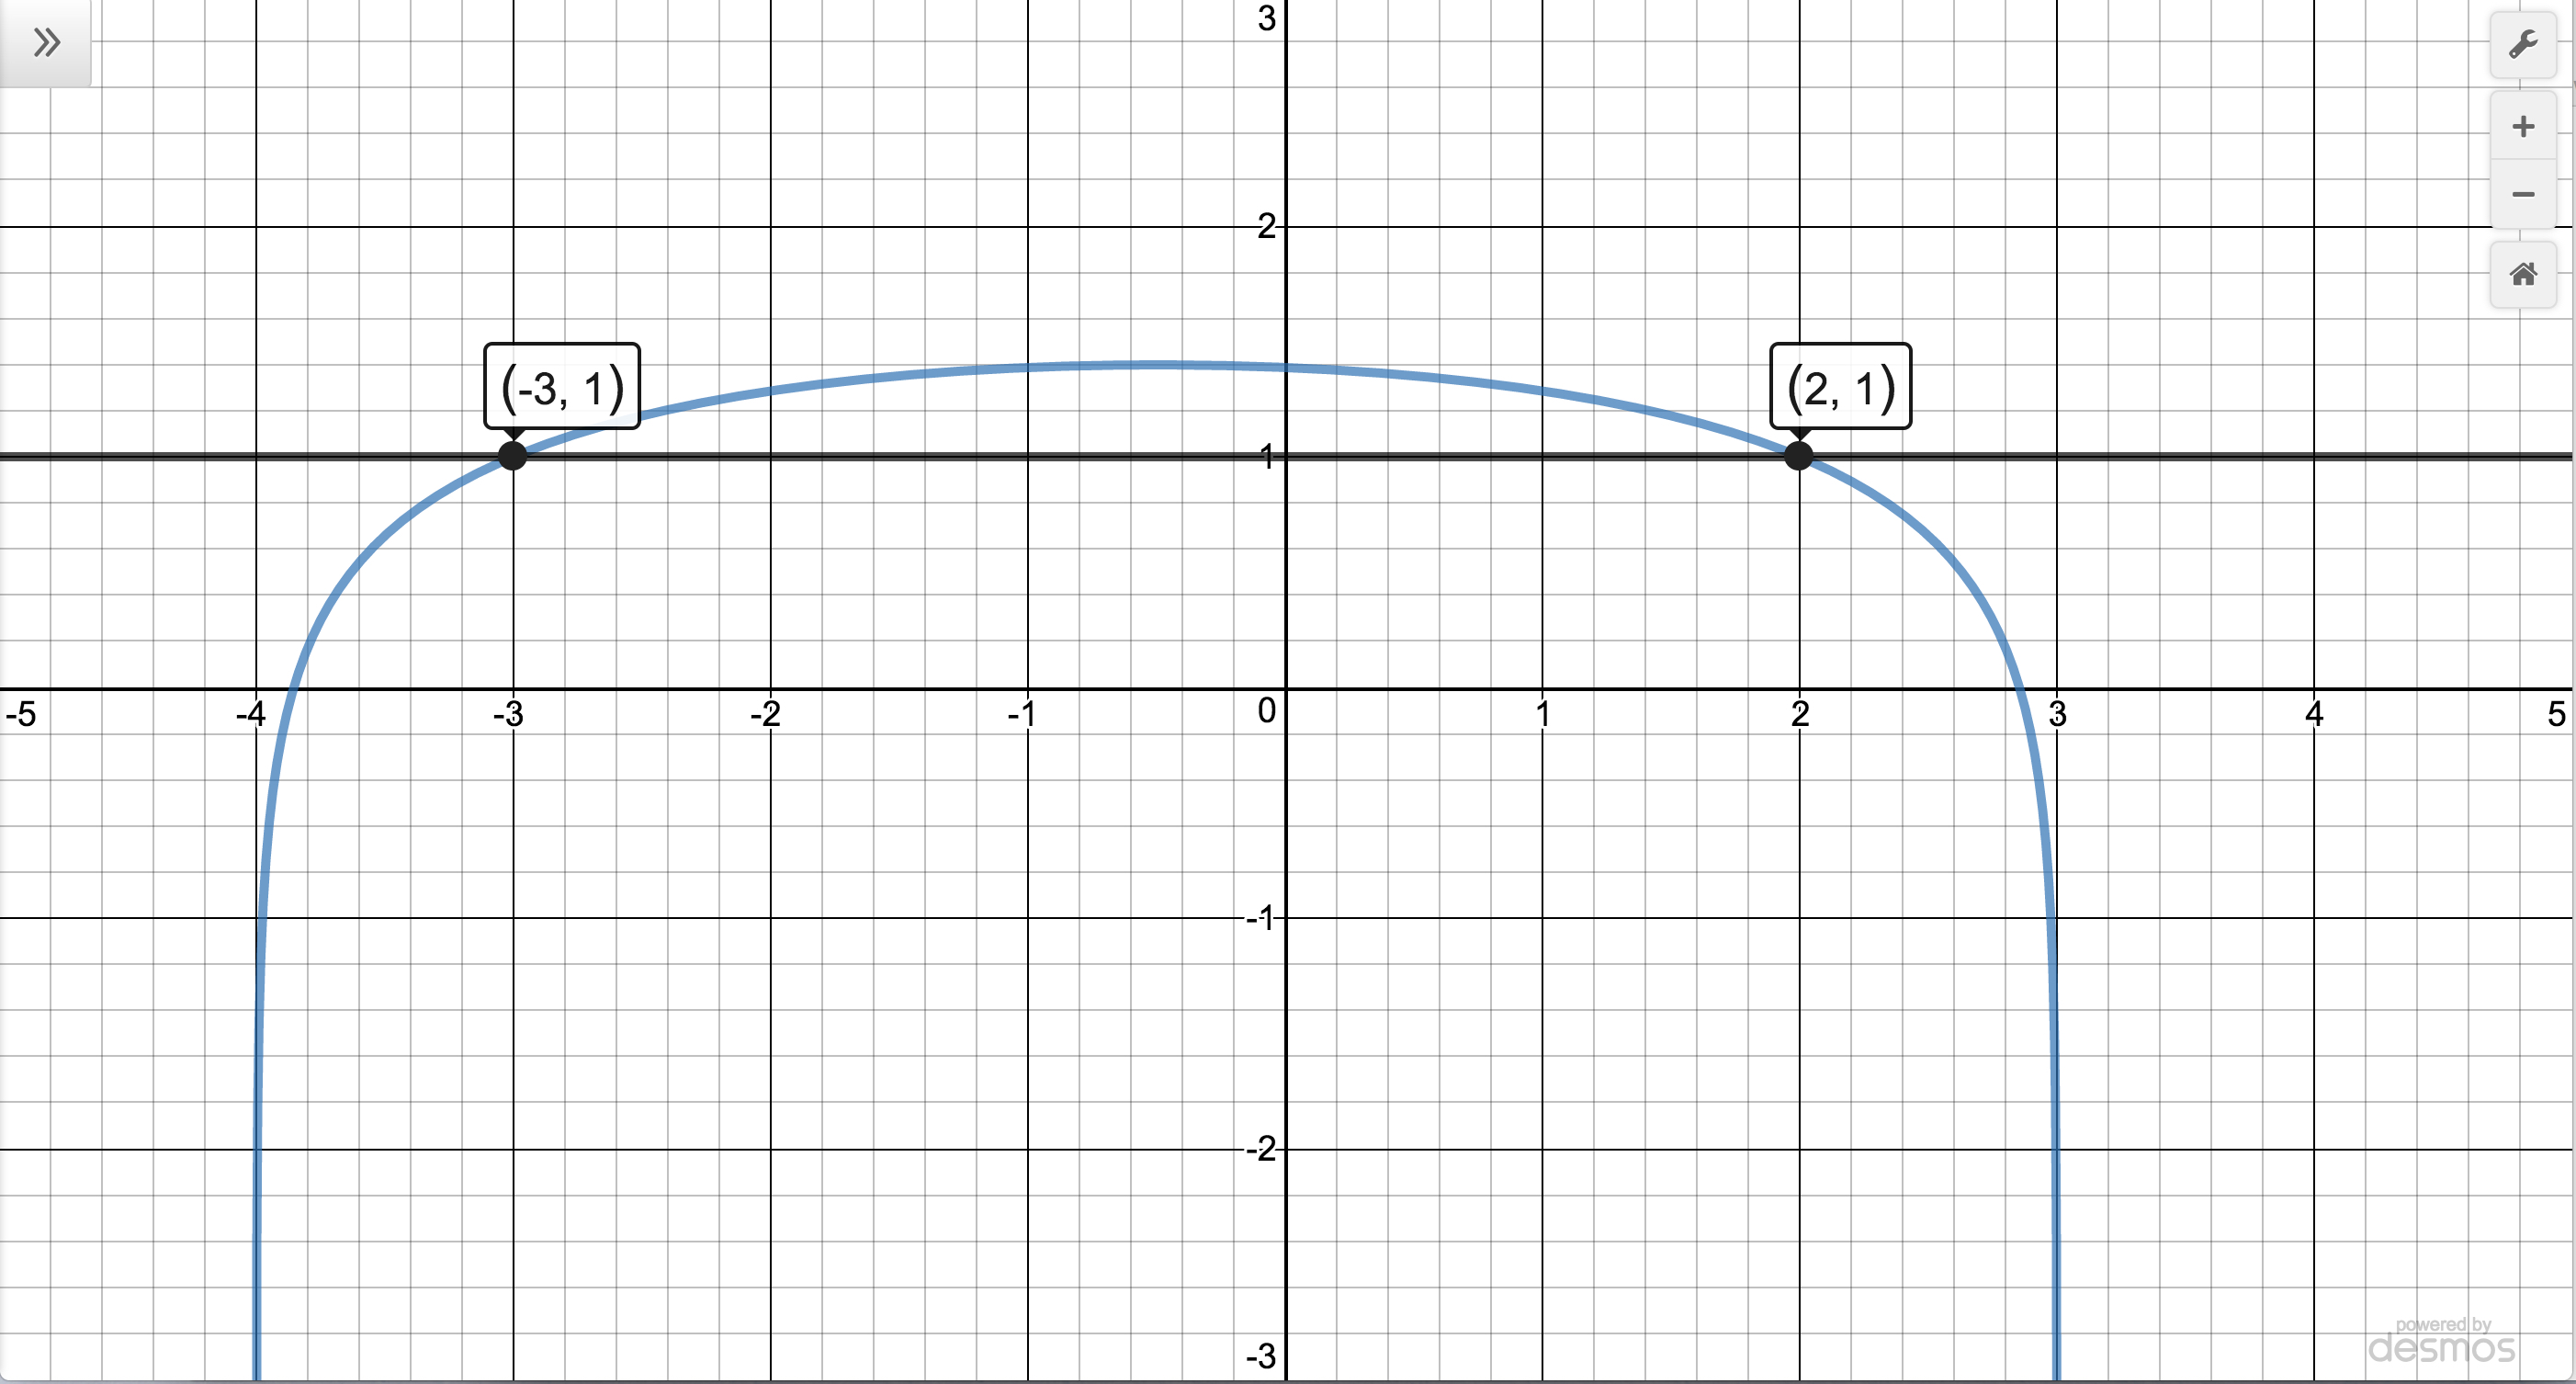
\includegraphics[width=3in]{./LogarithmicEquationsandInequalitiesGraphics/LogEqnEx03.jpg} &

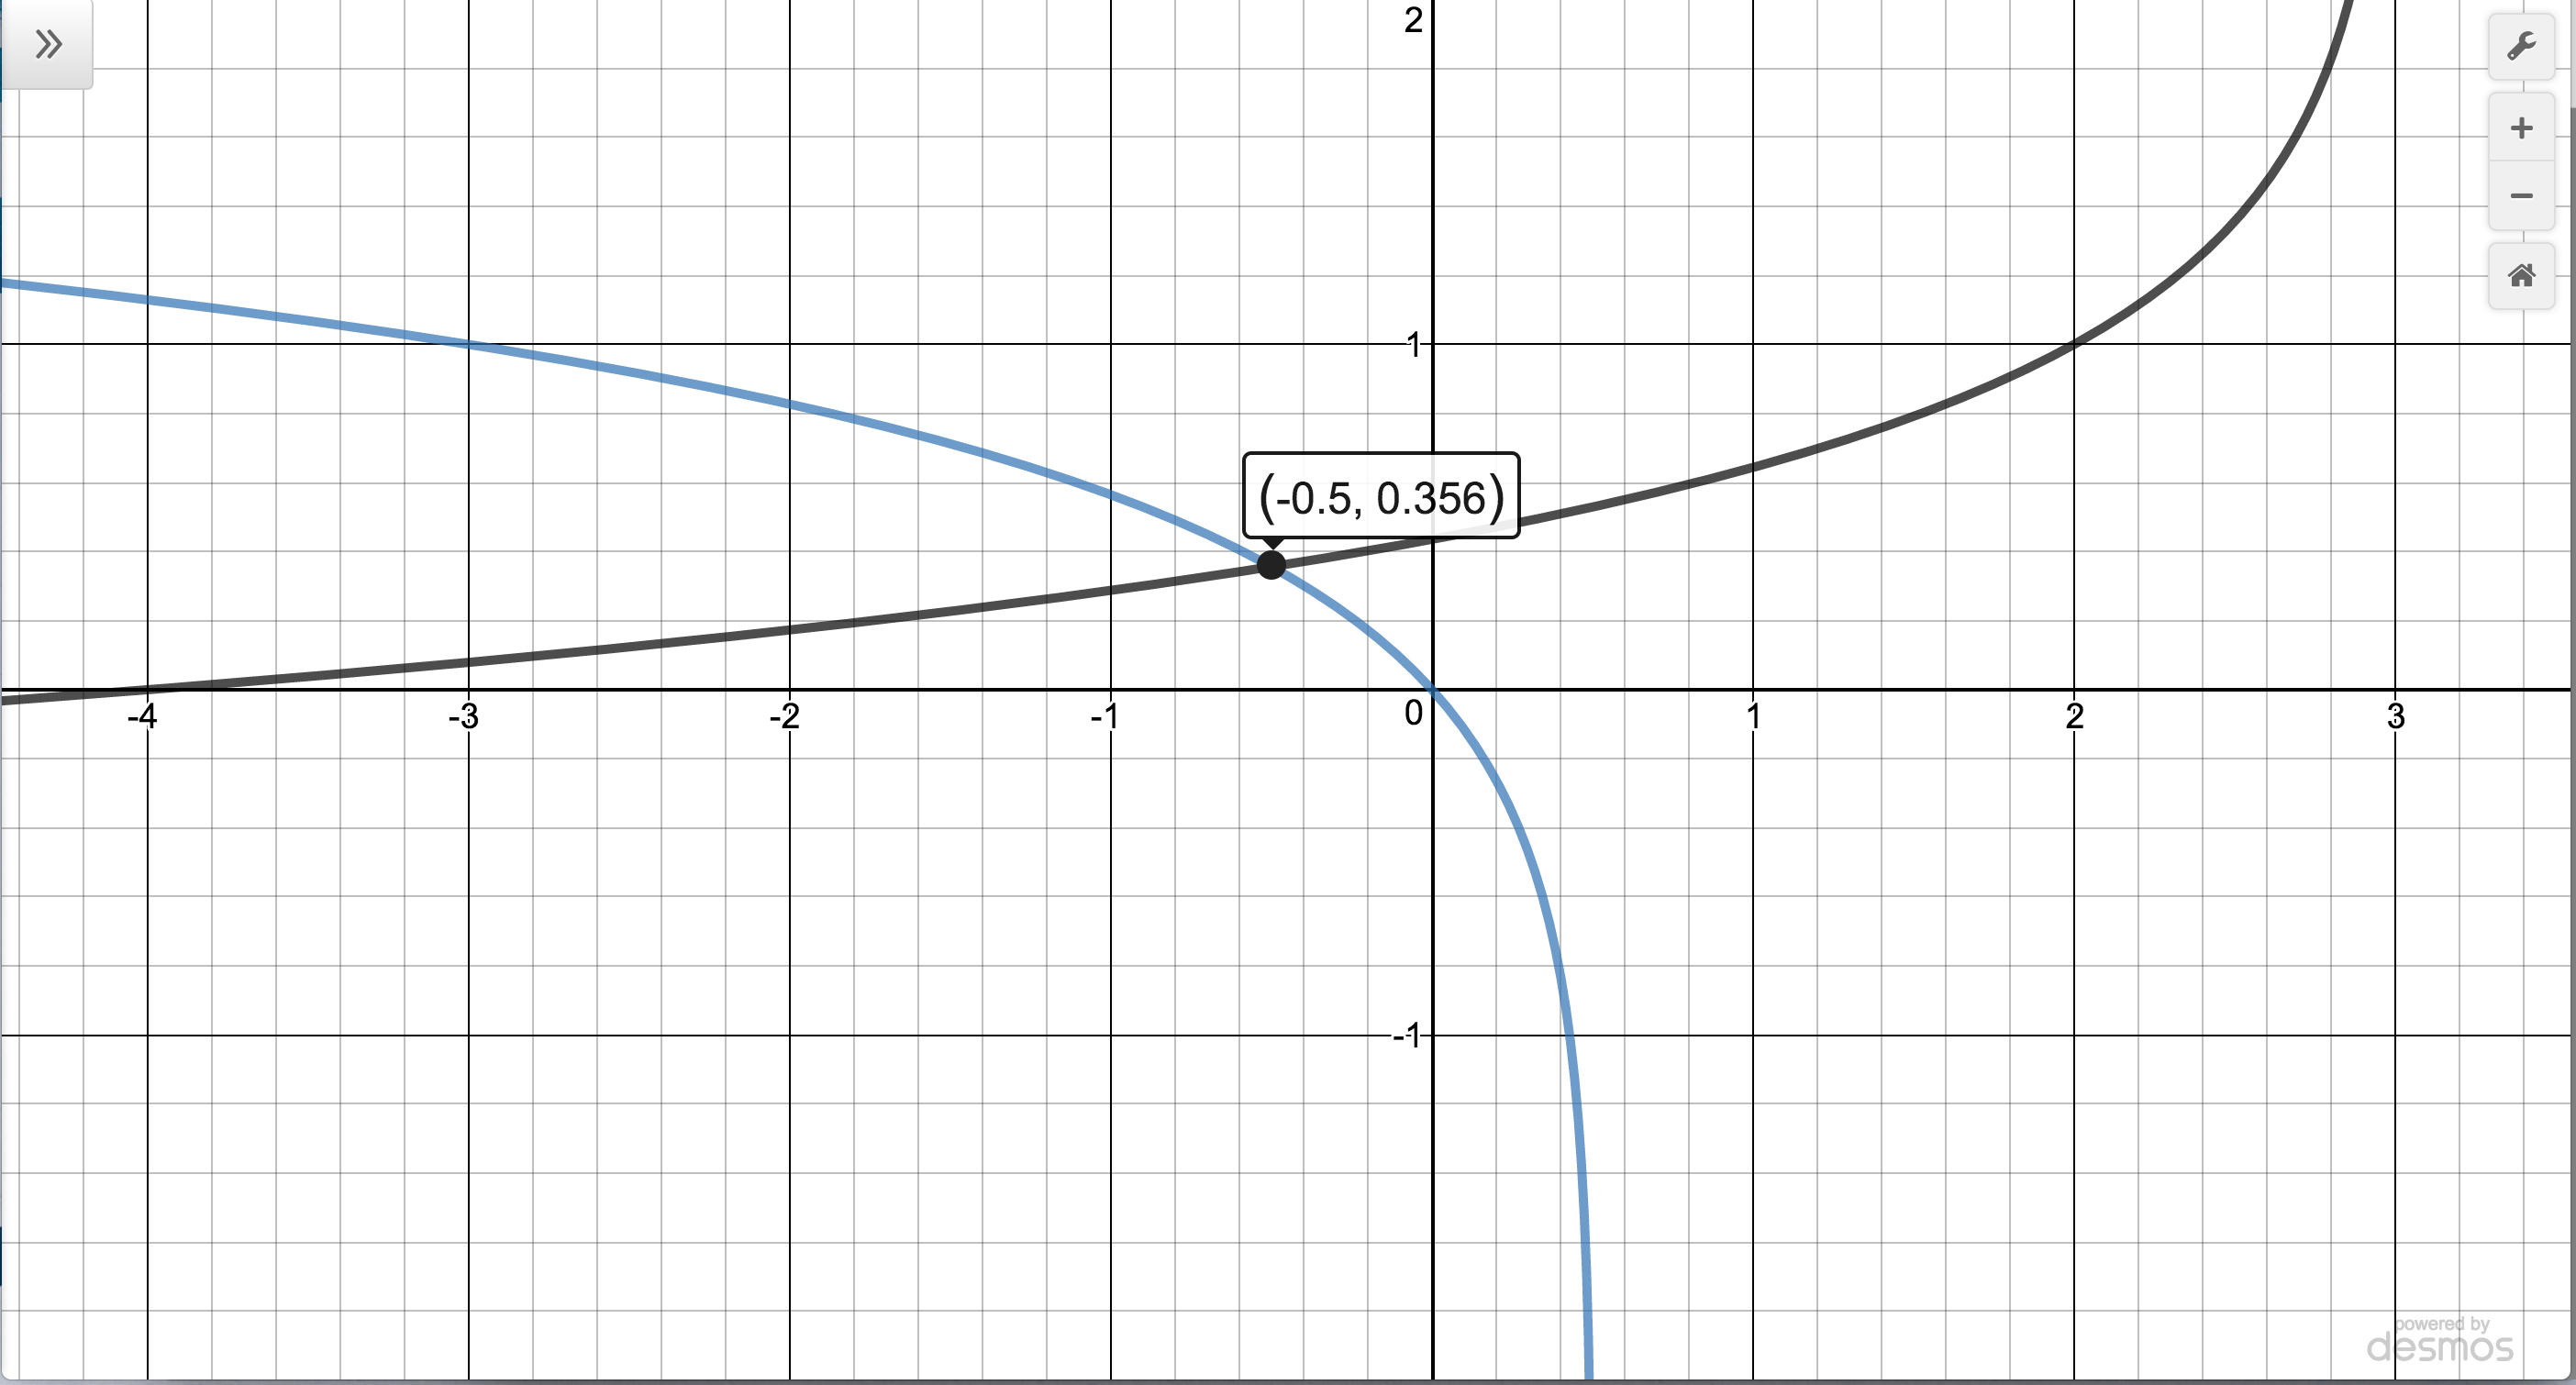
\includegraphics[width=3in]{./LogarithmicEquationsandInequalitiesGraphics/LogEqnEx04.jpg}  \\

Checking $\log_{6}(x+4) + \log_{6}(3-x) = 1$
 
 &
 
 Checking $\log_{7}(1-2t) = 1 - \log_{7}(3-t)$
 
\end{tabular}

\end{center}

\item Our first step in solving  $\log_{2}(x+3) = \log_{2}(6-x)+3$ is to gather the logarithms to one side of of the equation: $\log_{2}(x+3) - \log_{2}(6-x) = 3$.


\smallskip


The  Quotient Rule gives $\log_{2}\left(\frac{x+3}{6-x}\right) = 3$ which, as an exponential equation is $2^{3} = \frac{x+3}{6-x}$. 

\smallskip

Clearing denominators, we get $8(6-x) = x+3$, which reduces to  $x = 5$. 

\smallskip

Using the change of base once again, we graph $f(x) = \frac{\ln(x+3)}{\ln(2)}$ and $g(x) =  \frac{\ln(6-x)}{\ln(2)} + 3$ and find they intersect at $x=5$.


\item Our first step in solving $1 + 2 \log_{4}(t+1) = 2 \log_{2}(t)$ is to gather the logs on one side of the equation.  We obtain  $1 = 2 \log_{2}(t) - 2 \log_{4}(t+1)$ but find we need a common base to combine the logs.

\smallskip

Since $4$ is a power of $2$, we use change of base to convert  $\log_{4}(t+1) = \frac{\log_{2}(t+1)}{\log_{2}(4)} = \frac{1}{2} \log_{2}(t+1)$.  Hence, our original equation becomes  

\[ \begin{array}{rclr}

1 & = & 2 \log_{2}(t) - 2 \left(\frac{1}{2} \log_{2}(t+1)\right) & \\ [2pt]
1 &= & 2\log_{2}(t) - \log_{2}(t+1) & \\ [2pt]
1 & = & \log_{2}\left(t^2\right) - \log_{2}(t+1) & \text{Power Rule} \\ [6pt]
1 & = & \log_{2}\left( \dfrac{t^{2}}{t+1}\right) & \text{Quotient Rule} \\ \end{array}\]

Rewriting $1 = \log_{2}\left( \frac{t^{2}}{t+1}\right)$ in exponential form gives  $ \frac{t^{2}}{t+1} = 2$ or $t^2 -2t-2 = 0$.  Using the quadratic formula, we obtain  $t = 1 \pm \sqrt{3}$.

One last time, we use the change of base formula and graph  $f(t) = 1 + \frac{2\ln(t+1)}{\ln(4)}$ and $g(t) = \frac{2 \ln(t)}{\ln(2)}$.   We see the graphs intersect only at $t \approx 2.732 \approx 1 + \sqrt{3}$.  

\smallskip

Note the solution $t = 1 - \sqrt{3} < 0$ Hence if substituted into the original equation, the term $2 \log_{2}\left(1 - \sqrt{3}\right)$ is undefined, which explains why the graphs below intersect only once.

\begin{center}

\begin{tabular}{cc}

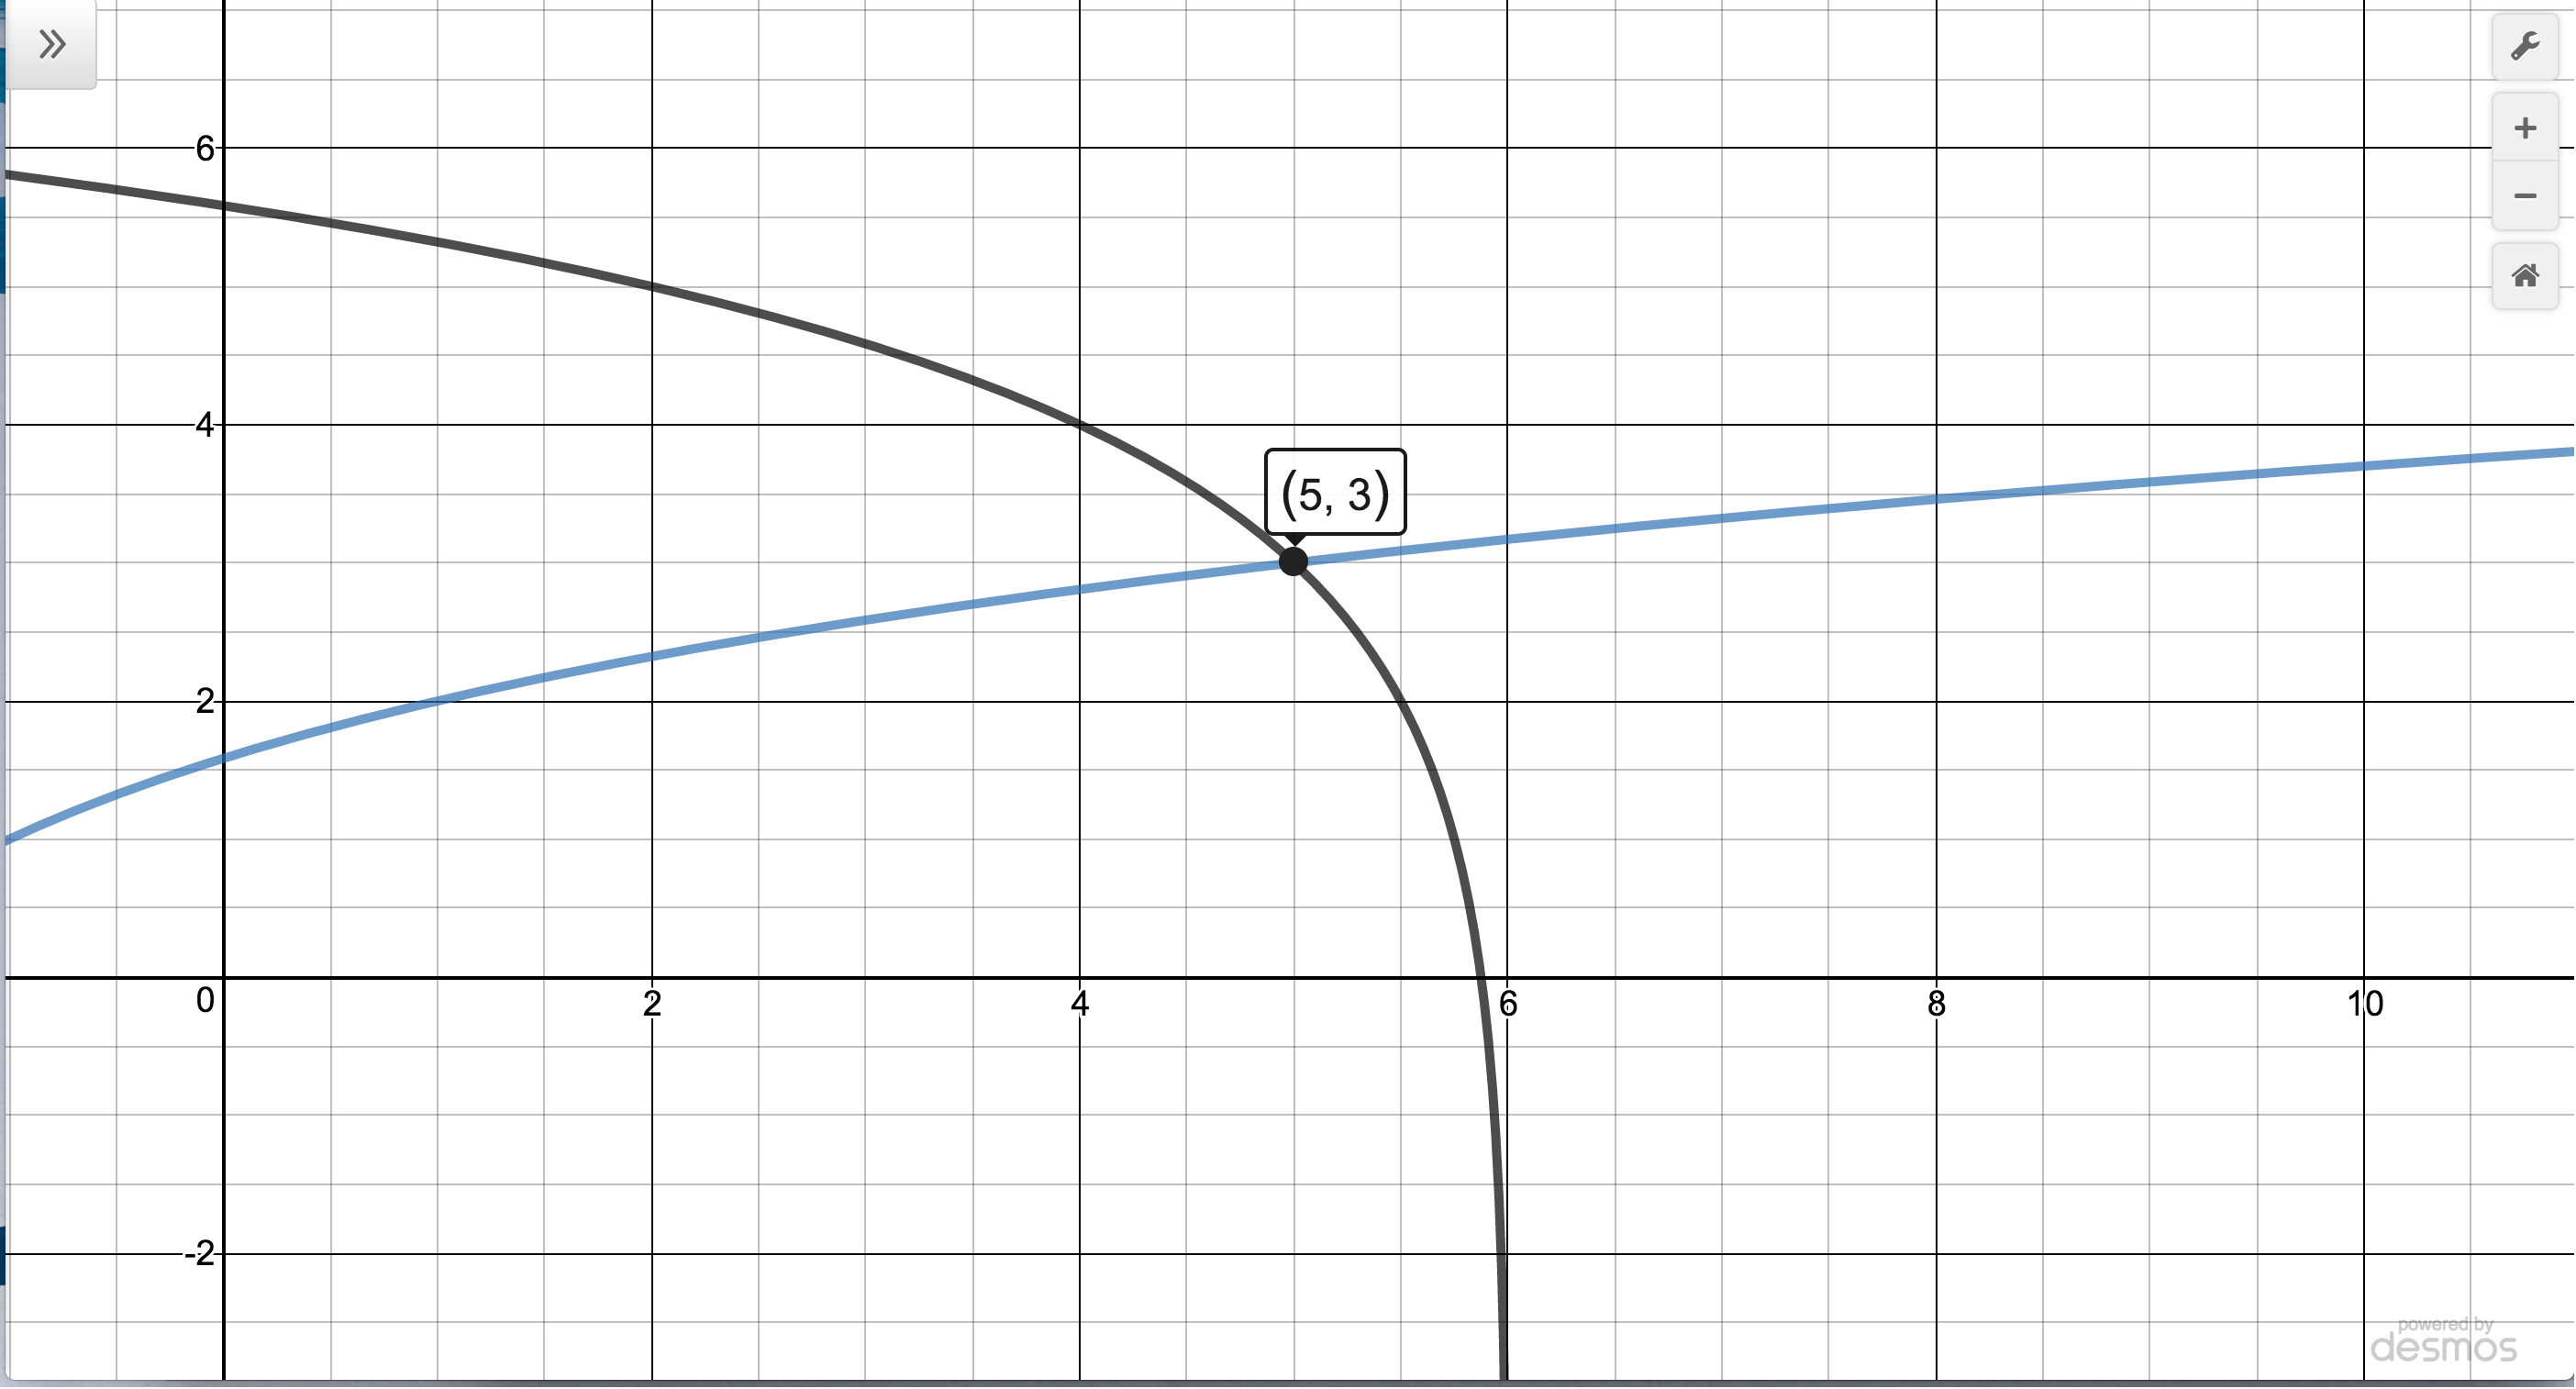
\includegraphics[width=3in]{./LogarithmicEquationsandInequalitiesGraphics/LogEqnEx05.jpg} &

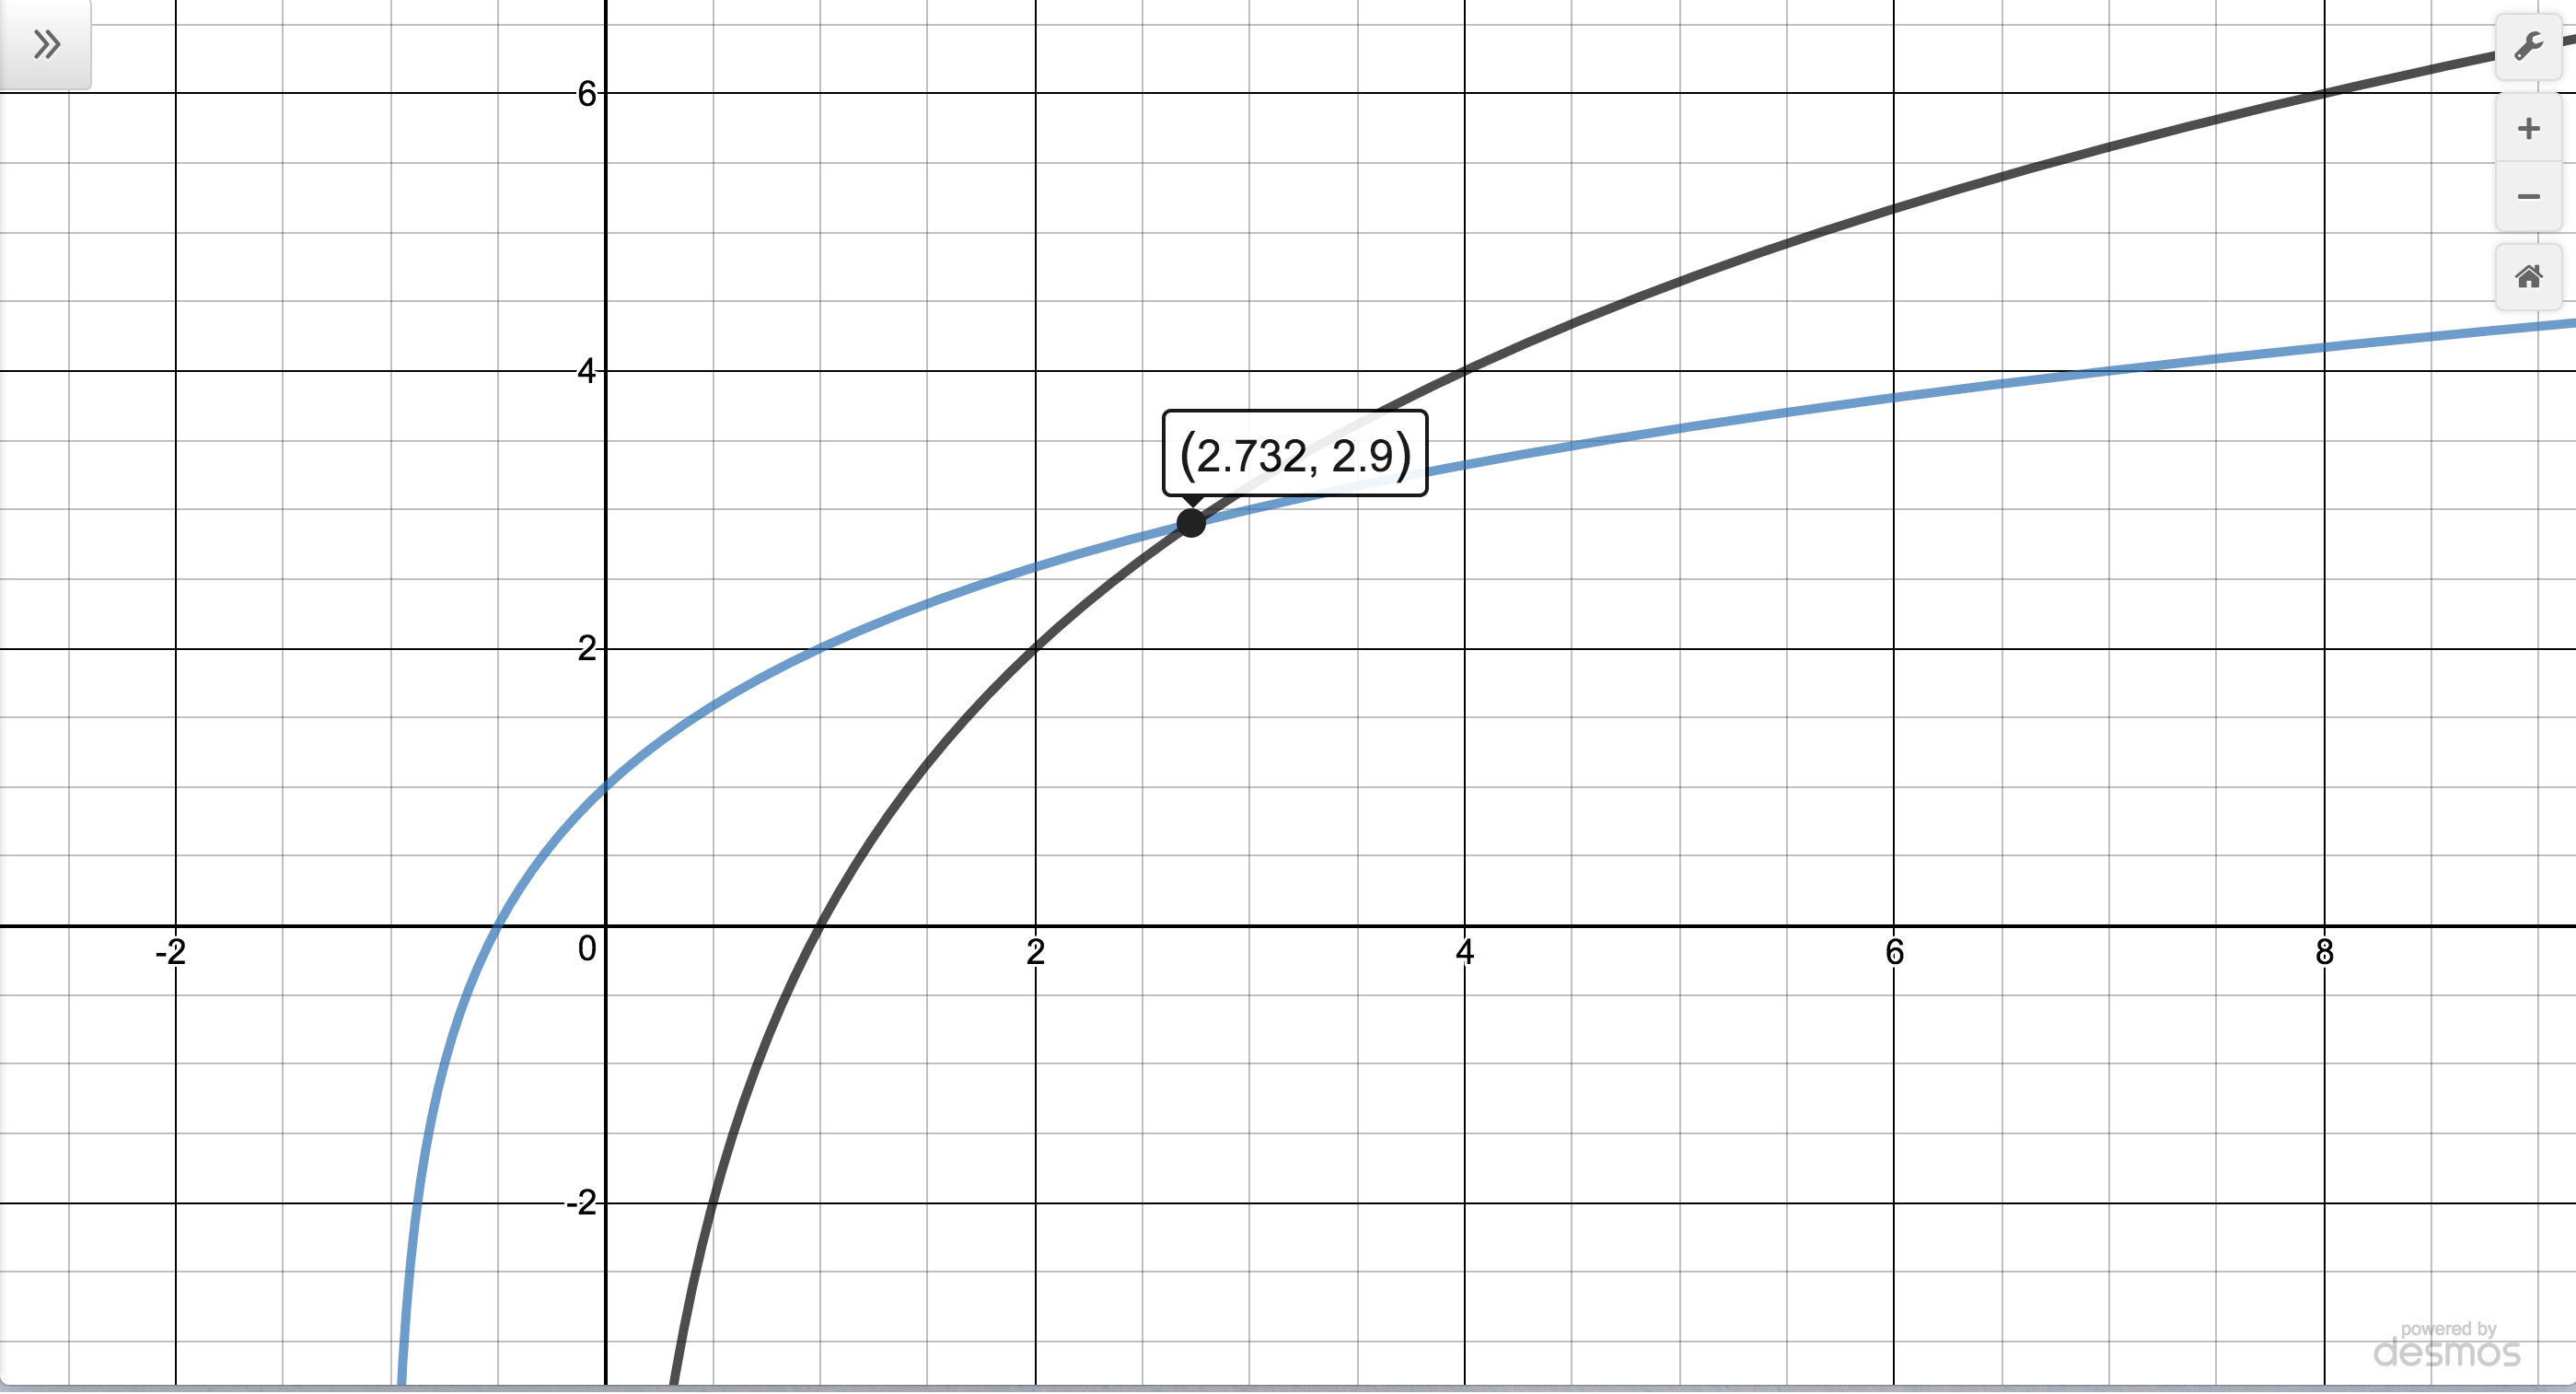
\includegraphics[width=3in]{./LogarithmicEquationsandInequalitiesGraphics/LogEqnEx06.jpg}  \\

Checking $\log_{2}(x+3) = \log_{2}(6-x)+3$
 
 &
 
 Checking $1 + 2 \log_{4}(t+1) = 2 \log_{2}(t)$
 
\end{tabular}

\end{center}
\end{enumerate}

\qed
\end{example}

If nothing else,  Example \ref{LogEqnsEx1} demonstrates the importance of checking for extraneous solutions\footnote{Recall that an extraneous solution is an answer obtained analytically which does not satisfy the original equation.} when solving equations involving logarithms.  Even though we checked our answers graphically, extraneous solutions are easy to spot:  any supposed solution which causes the argument of a logarithm to be negative must be discarded.  

\smallskip

While identifying extraneous solutions is important, it is equally important to understand which machinations create the opportunity for extraneous solutions to appear.  In the case of Example \ref{LogEqnsEx1}, extraneous solutions, by and large, result from using the Power, Product, or Quotient Rules.  We encourage the reader to take the time to track each extraneous solution found in  Example \ref{LogEqnsEx1}  backwards through the solution process to see at precisely which step it fails to be a solution.

\smallskip

As with the equations in Example \ref{expeqnsex1}, much can be learned from checking all of the answers in Example \ref{LogEqnsEx1} analytically.  We leave this to the reader and turn our attention to inequalities involving logarithmic functions.  Since logarithmic functions are continuous on their domains, we can use sign diagrams.  

\smallskip

\begin{example}  Solve the following inequalities.  Check your answer graphically using a calculator.
\label{logineq}

\begin{multicols}{3}

\begin{enumerate}

\item  $\dfrac{1}{\ln(x)+1} \leq 1$

\item  $\left(\log_{2}(x)\right)^2 < 2 \log_{2}(x) + 3$

\item  $t \log(t+1) \geq t$


\end{enumerate}

\end{multicols}


{\bf Solution.}  

\begin{enumerate}

\item  We start solving $\frac{1}{\ln(x)+1} \leq 1$ by getting $0$ on one side of the inequality: $\frac{1}{\ln(x)+1}  - 1 \leq 0$.  

\smallskip

Getting a common denominator yields $\frac{1}{\ln(x)+1}  - \frac{\ln(x)+1}{\ln(x)+1} \leq 0$ which reduces to $\frac{-\ln(x)}{\ln(x)+1} \leq 0$, or $ \frac{\ln(x)}{\ln(x)+1} \geq 0$.  

\smallskip

We define $r(x) = \frac{\ln(x)}{\ln(x)+1}$ and set about finding the domain and the zeros of $r$.  Due to the appearance of the term $\ln(x)$, we require  $x > 0$.  In order to keep the denominator away from zero, we solve $\ln(x)+1 = 0$ so $\ln(x) = -1$, so $x = e^{-1} = \frac{1}{e}$.  Hence, the domain of $r$ is $\left(0, \frac{1}{e}\right) \cup \left(\frac{1}{e}, \infty\right)$. 

\smallskip

To find the zeros of $r$, we set $r(x) = \frac{\ln(x)}{\ln(x)+1} = 0$ so that $\ln(x) = 0$, and we find $x = e^{0} = 1$.  


\smallskip

In order to determine test values for $r$ without resorting to the calculator, we need to find numbers between $0$, $\frac{1}{e}$, and $1$ which have a base of $e$.  Since $e \approx 2.718 > 1$, $0 < \frac{1}{e^2} < \frac{1}{e} < \frac{1}{\sqrt{e}} < 1 < e$.  

\smallskip

To determine the sign of $r\left( \frac{1}{e^2} \right)$, note $\ln\left(\frac{1}{e^2}\right) = \ln\left(e^{-2}\right) = -2$. Hence, $r\left( \frac{1}{e^2} \right) = \frac{-2}{-2+1} = 2 > 0$.  The rest of the test values are determined similarly.   


\smallskip

From our sign diagram, we find $r(x) \geq 0$ on $\left(0, \frac{1}{e}\right) \cup [1, \infty)$, which is our solution. 


\smallskip

Graphing $f(x) =  \frac{1}{\ln(x)+1}$ and $g(x) = 1$, we see the graph of $f$ is below the graph of $g$ on these intervals, and that the graphs intersect at $x=1$.

\begin{center}

\begin{tabular}{cc}

\begin{mfpic}[10]{-6}{6}{-2}{2}
\arrow \polyline{(-6,0),(6,0)}
\xmarks{-2,2}
\scriptsize
\tlpointsep{6pt}
\normalsize
\tlabel[cc](-6,-1){$0$}
\tlabel[cc](-4,1){$(+)$}
\tlabel[cc](-2,-1){$\frac{1}{e}$}
\tlabel[cc](-2,1){\textinterrobang}
\tlabel[cc](0,1){$(-)$}
\tlabel[cc](2,-1){$1$}
\tlabel[cc](2,1){$0$}
\tlabel[cc](4,1){$(+)$}
\pointfillfalse
\point[4pt]{(-6,0)}
\end{mfpic} 

& 

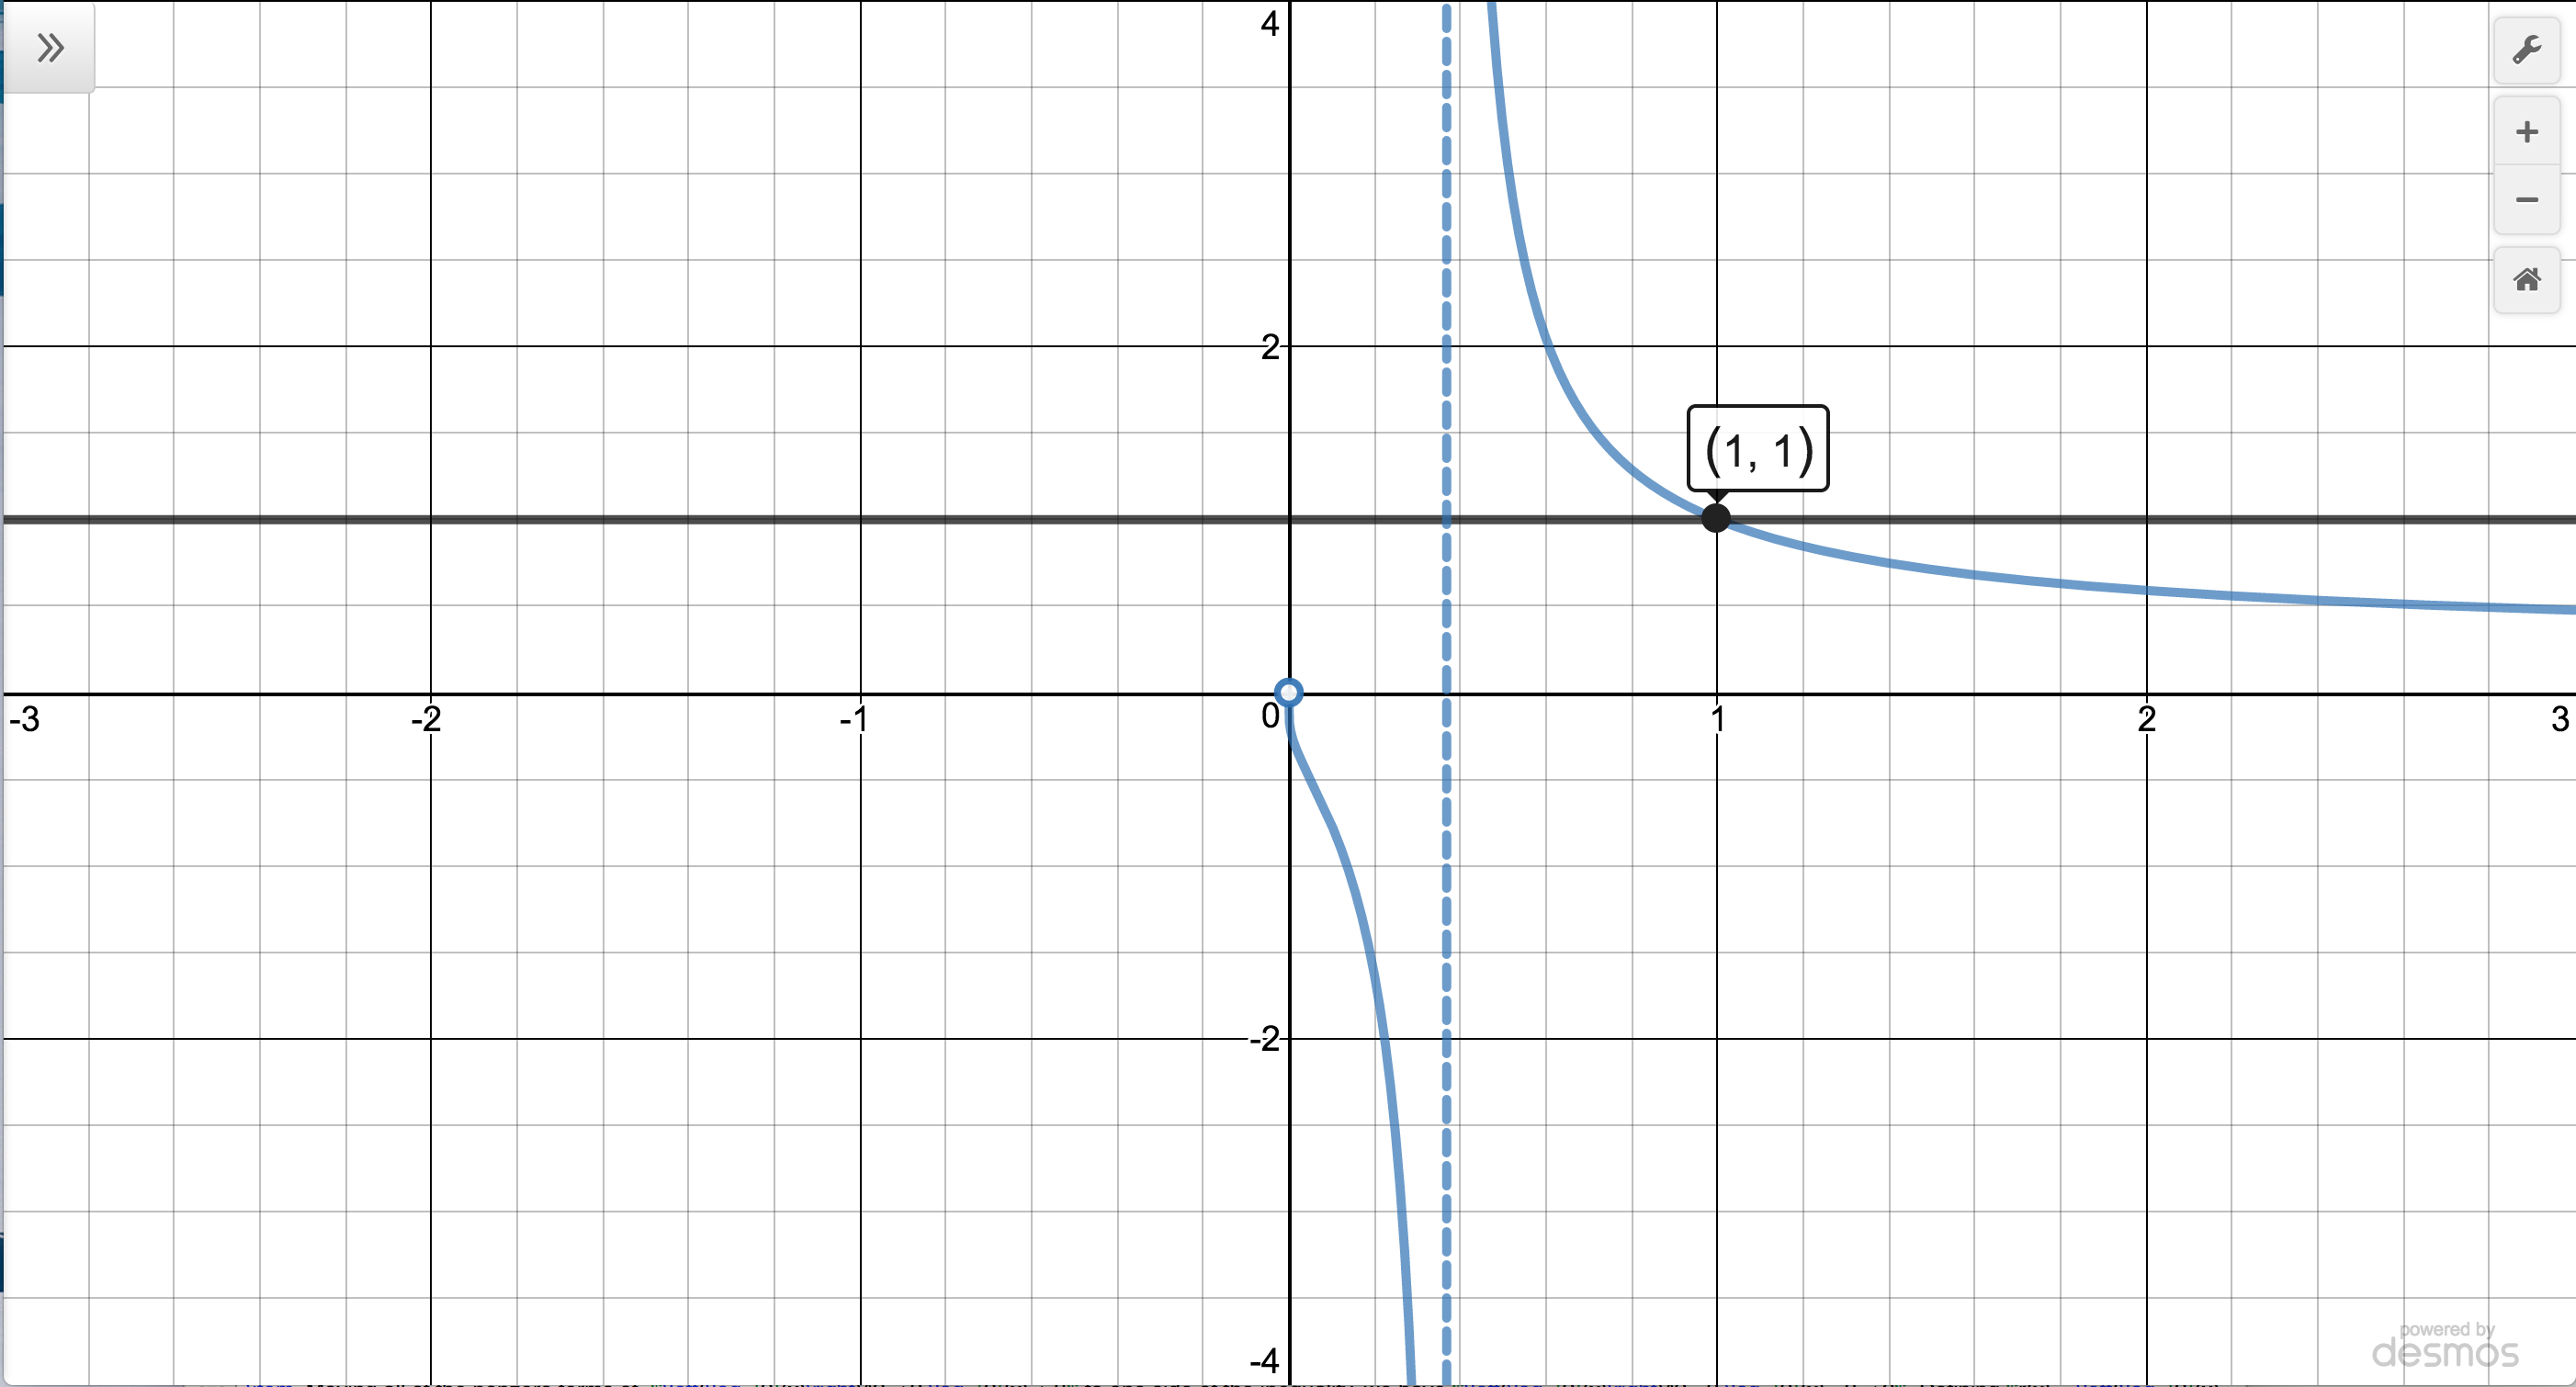
\includegraphics[width=3in]{./LogarithmicEquationsandInequalitiesGraphics/LogEqnEx07.jpg} \\

A sign diagram for $r(x) = \dfrac{\ln(x)}{\ln(x)+1}$

&

Checking  $\dfrac{1}{\ln(x)+1} \leq 1$



\end{tabular}

\end{center}


\item  Moving all of the nonzero terms of  $\left(\log_{2}(x)\right)^2 < 2 \log_{2}(x) + 3$ to one side of the inequality in order to make use of a sign diagram, we have $\left(\log_{2}(x)\right)^2 - 2 \log_{2}(x) - 3 < 0$. 

\smallskip

Defining $r(x) = \left(\log_{2}(x)\right)^2 - 2 \log_{2}(x) - 3$, we get the domain of $r$ is $(0, \infty)$, due to the presence of the logarithm.  To find the zeros of $r$, we set $r(x) =\left(\log_{2}(x)\right)^2 - 2 \log_{2}(x) - 3= 0$ which we identify as a  `quadratic in disguise.'  

\smallskip

Setting $u = \log_{2}(x)$, our equation becomes $u^2-2u-3 = 0$.  Factoring   gives us $u=-1$ and $u=3$.  Since $u = \log_{2}(x)$, we get $\log_{2}(x) = -1$, or $x = 2^{-1} = \frac{1}{2}$, and $\log_{2}(x) = 3$, which gives  $x = 2^{3} = 8$.  

\smallskip

We use test values which are powers of $2$: $0 < \frac{1}{4} < \frac{1}{2} < 1 < 8 < 16$ to create the sign diagram below.  From our sign diagram, we see $r(x)< 0$, which corresponds to our solution,  on $\left(\frac{1}{2}, 8 \right)$. 

\smallskip

Geometrically, the graph of $f(x)= \left(\frac{\ln(x)}{\ln(2)}\right)^2$ is below the graph of $y = g(x) = \frac{2 \ln(x)}{\ln(2)} + 3$ on $\left(\frac{1}{2}, 8 \right)$.

\begin{center}

\begin{tabular}{m{2in}c}

\begin{mfpic}[10]{-6}{6}{-2}{2}
\arrow \polyline{(-6,0),(6,0)}
\xmarks{-2,2}
\scriptsize
\tlpointsep{6pt}
\normalsize
\tlabel[cc](-6,-1){$0$}
\tlabel[cc](-4,1){$(+)$}
\tlabel[cc](-2,-1){$\frac{1}{2}$}
\tlabel[cc](-2,1){$0$}
\tlabel[cc](0,1){$(-)$}
\tlabel[cc](2,-1){$8$}
\tlabel[cc](2,1){$0$}
\tlabel[cc](4,1){$(+)$}
\pointfillfalse
\point[4pt]{(-6,0)}
\end{mfpic} 

& 

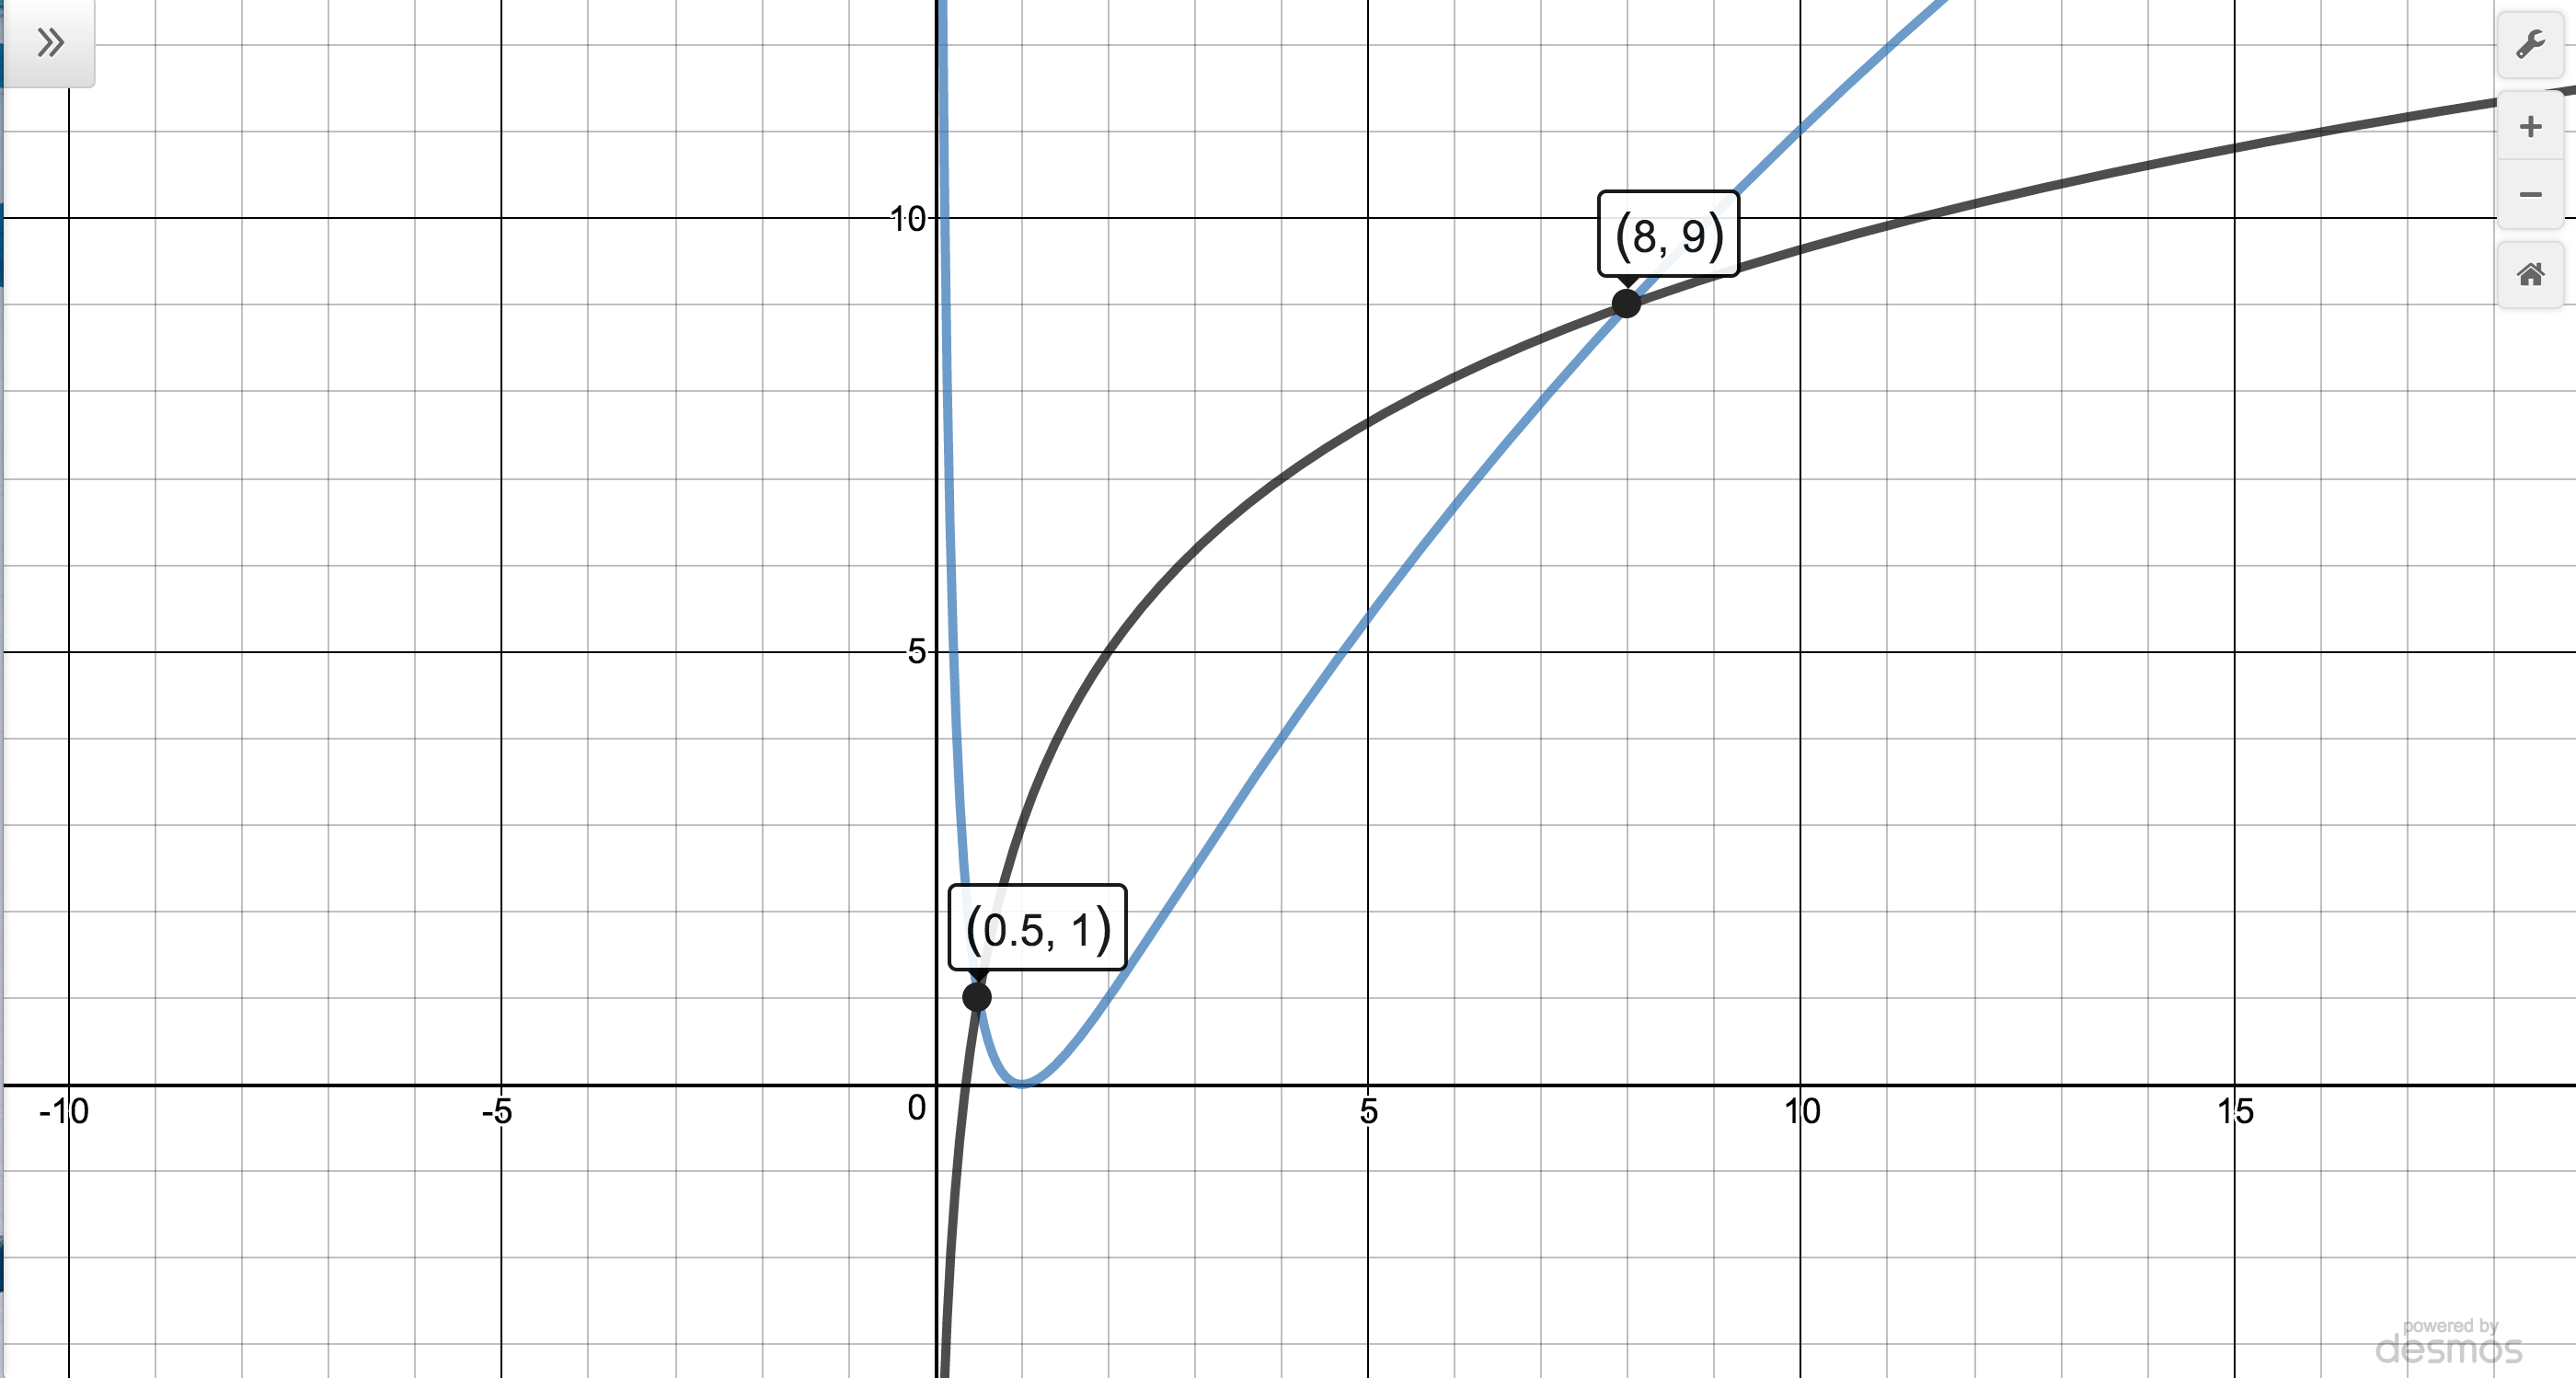
\includegraphics[width=3in]{./LogarithmicEquationsandInequalitiesGraphics/LogEqnEx08.jpg} \\

A sign diagram for 

&

Checking $\left(\log_{2}(x)\right)^2 < 2 \log_{2}(x) + 3$ \\

 $r(x) = \left(\log_{2}(x)\right)^2 - 2 \log_{2}(x) - 3$
 
 & \\

\end{tabular}

\end{center}



\item  We begin to solve $t \log(t+1) \geq t$ by subtracting $t$ from both sides to get $t \log(t+1)  - t \geq 0$.  

\smallskip

We define $r(t) = t \log(t+1)  - t $ and due to the presence of the logarithm, we require $t > -1$.  

\smallskip

To find the zeros of $r$, we set $r(t) = t \log(t+1)  - t = 0$.  Factoring, we get $t \left(\log(t+1) - 1\right) = 0$, which gives $t=0$ or $\log(t+1) - 1=0$.  

\smallskip

From $\log(t+1) - 1=0$ we get   $\log(t+1) = 1$, which we  rewrite as  $t+1 = 10^{1}$. Hence,   $t = 9$.  

\smallskip

We select test values $t$ so that $t+1$ is a power of $10$. Using $-1 < -0.9 < 0 < \sqrt{10} -1 < 9 < 99$,   our sign diagram gives the solution as $(-1,0] \cup [9, \infty)$. 

\smallskip

We find the graphs of  $y= f(t) = t \log(t+1)$  and $y=g(t) = t$ intersect at $t=0$ and $t=9$ with the graph of $f$ above the graph of $g$ on the given solution intervals.


\begin{center}

\begin{tabular}{m{2in}c}

\begin{mfpic}[10]{-6}{6}{-2}{2}
\arrow \polyline{(-6,0),(6,0)}
\xmarks{-2,2}
\scriptsize
\tlpointsep{4pt}
\normalsize
\tlabel[cc](-6,-1){$-1$}
\tlabel[cc](-4,1){$(+)$}
\tlabel[cc](-2,-1){$0$}
\tlabel[cc](-2,1){$0$}
\tlabel[cc](0,1){$(-)$}
\tlabel[cc](2,-1){$9$}
\tlabel[cc](2,1){$0$}
\tlabel[cc](4,1){$(+)$}
\pointfillfalse
\point[4pt]{(-6,0)}
\end{mfpic} 

& 


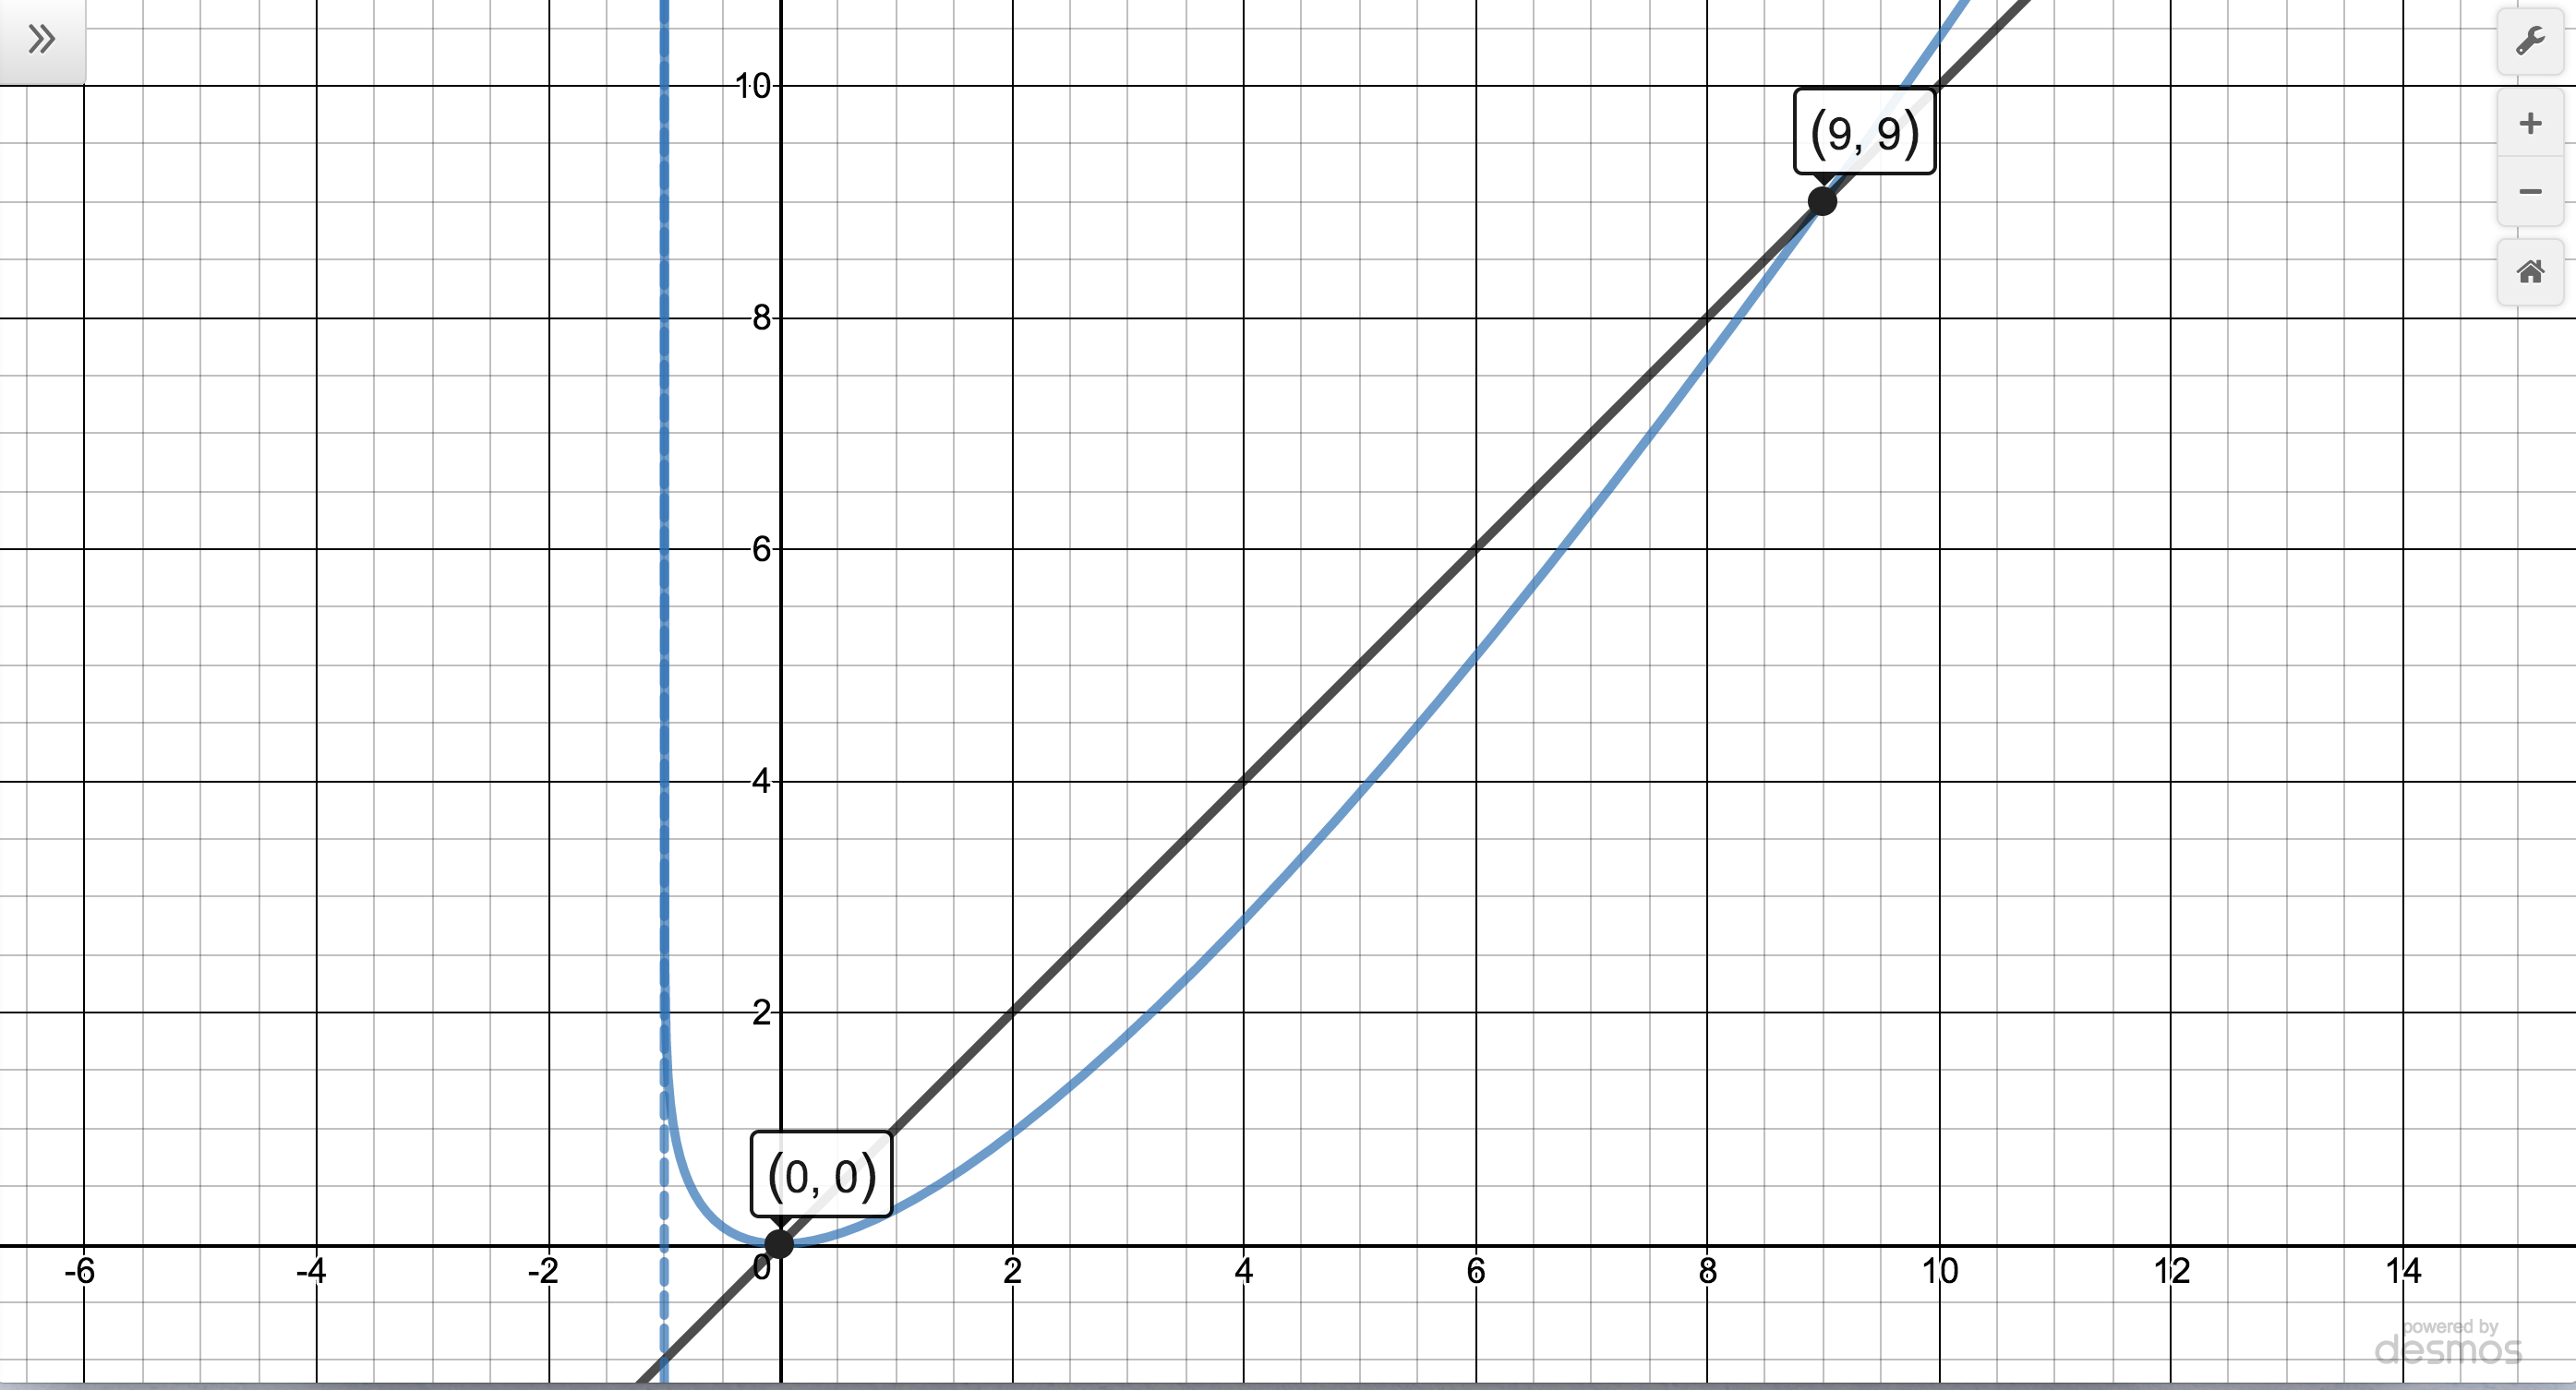
\includegraphics[width=3in]{./LogarithmicEquationsandInequalitiesGraphics/LogEqnEx09.jpg} \\

A sign diagram for   
&

Checking $t \log(t+1) \geq t$ \\

$r(t) = t \log(t+1)  - t $ & \\


\end{tabular}

\end{center}

\qed
\end{enumerate}
\end{example}

\smallskip

Our next example revisits the concept of pH first seen in Exercise \ref{pHexercise} in Section \ref{LogarithmicFunctions}.  


\begin{example}

In order to successfully breed Ippizuti fish the pH of a freshwater tank must be at least 7.8 but can be no more than 8.5.  Determine the corresponding range of hydrogen ion concentration, and check your answer using a calculator.

\smallskip

{\bf Solution.}  Recall from Exercise \ref{pHexercise} in Section \ref{LogarithmicFunctions} that $\text{pH} = -\log[\text{H}^{+}]$ where $[\text{H}^{+}]$ is the hydrogen ion concentration in moles per liter.  

\smallskip

We require $7.8 \leq -\log[\text{H}^{+}] \leq 8.5$ or $-8.5 \leq   \log[\text{H}^{+}] \leq -7.8$.  One way to proceed is to break this compound inequality into two inequalities, solve each using a sign diagram, and take the intersection of the solution sets.\footnote{Refer to page \pageref{intersectionunion} for a discussion of what this means.}  

\smallskip

On the other hand, we take advantage of the fact that $F(x) = 10^{x}$ is an increasing function, meaning that if $a \leq b \leq c$, then $10^{a} \leq 10^{b} \leq 10^{c}$.  This property allows us to solve our inequality in one step: from $-8.5 \leq   \log[\text{H}^{+}] \leq -7.8$, we get   $10^{-8.5} \leq   10^{\log[\text{H}^{+}]} \leq 10^{-7.8}$, so our solution is $ \leq   [\text{H}^{+}] \leq 10^{-7.8}$.  (Your Chemistry professor may want the answer written as $3.16 \times 10^{-9} \leq [\text{H}^{+}] \leq 1.58 \times 10^{-8}$.)  Using interval notation, our answer is $\left[10^{-8.5}, 10^{-7.8}\right]$.   

\smallskip

After \textit{very} carefully adjusting the viewing window on the graphing utility, we see the graph of $f(x) = -\log(x)$ lies between the lines $y = 7.8$ and $y = 8.5$ on the interval $[3.162 \times 10^{-9}, 1.5849 \times 10^{-8}]$.

\smallskip

\begin{center}

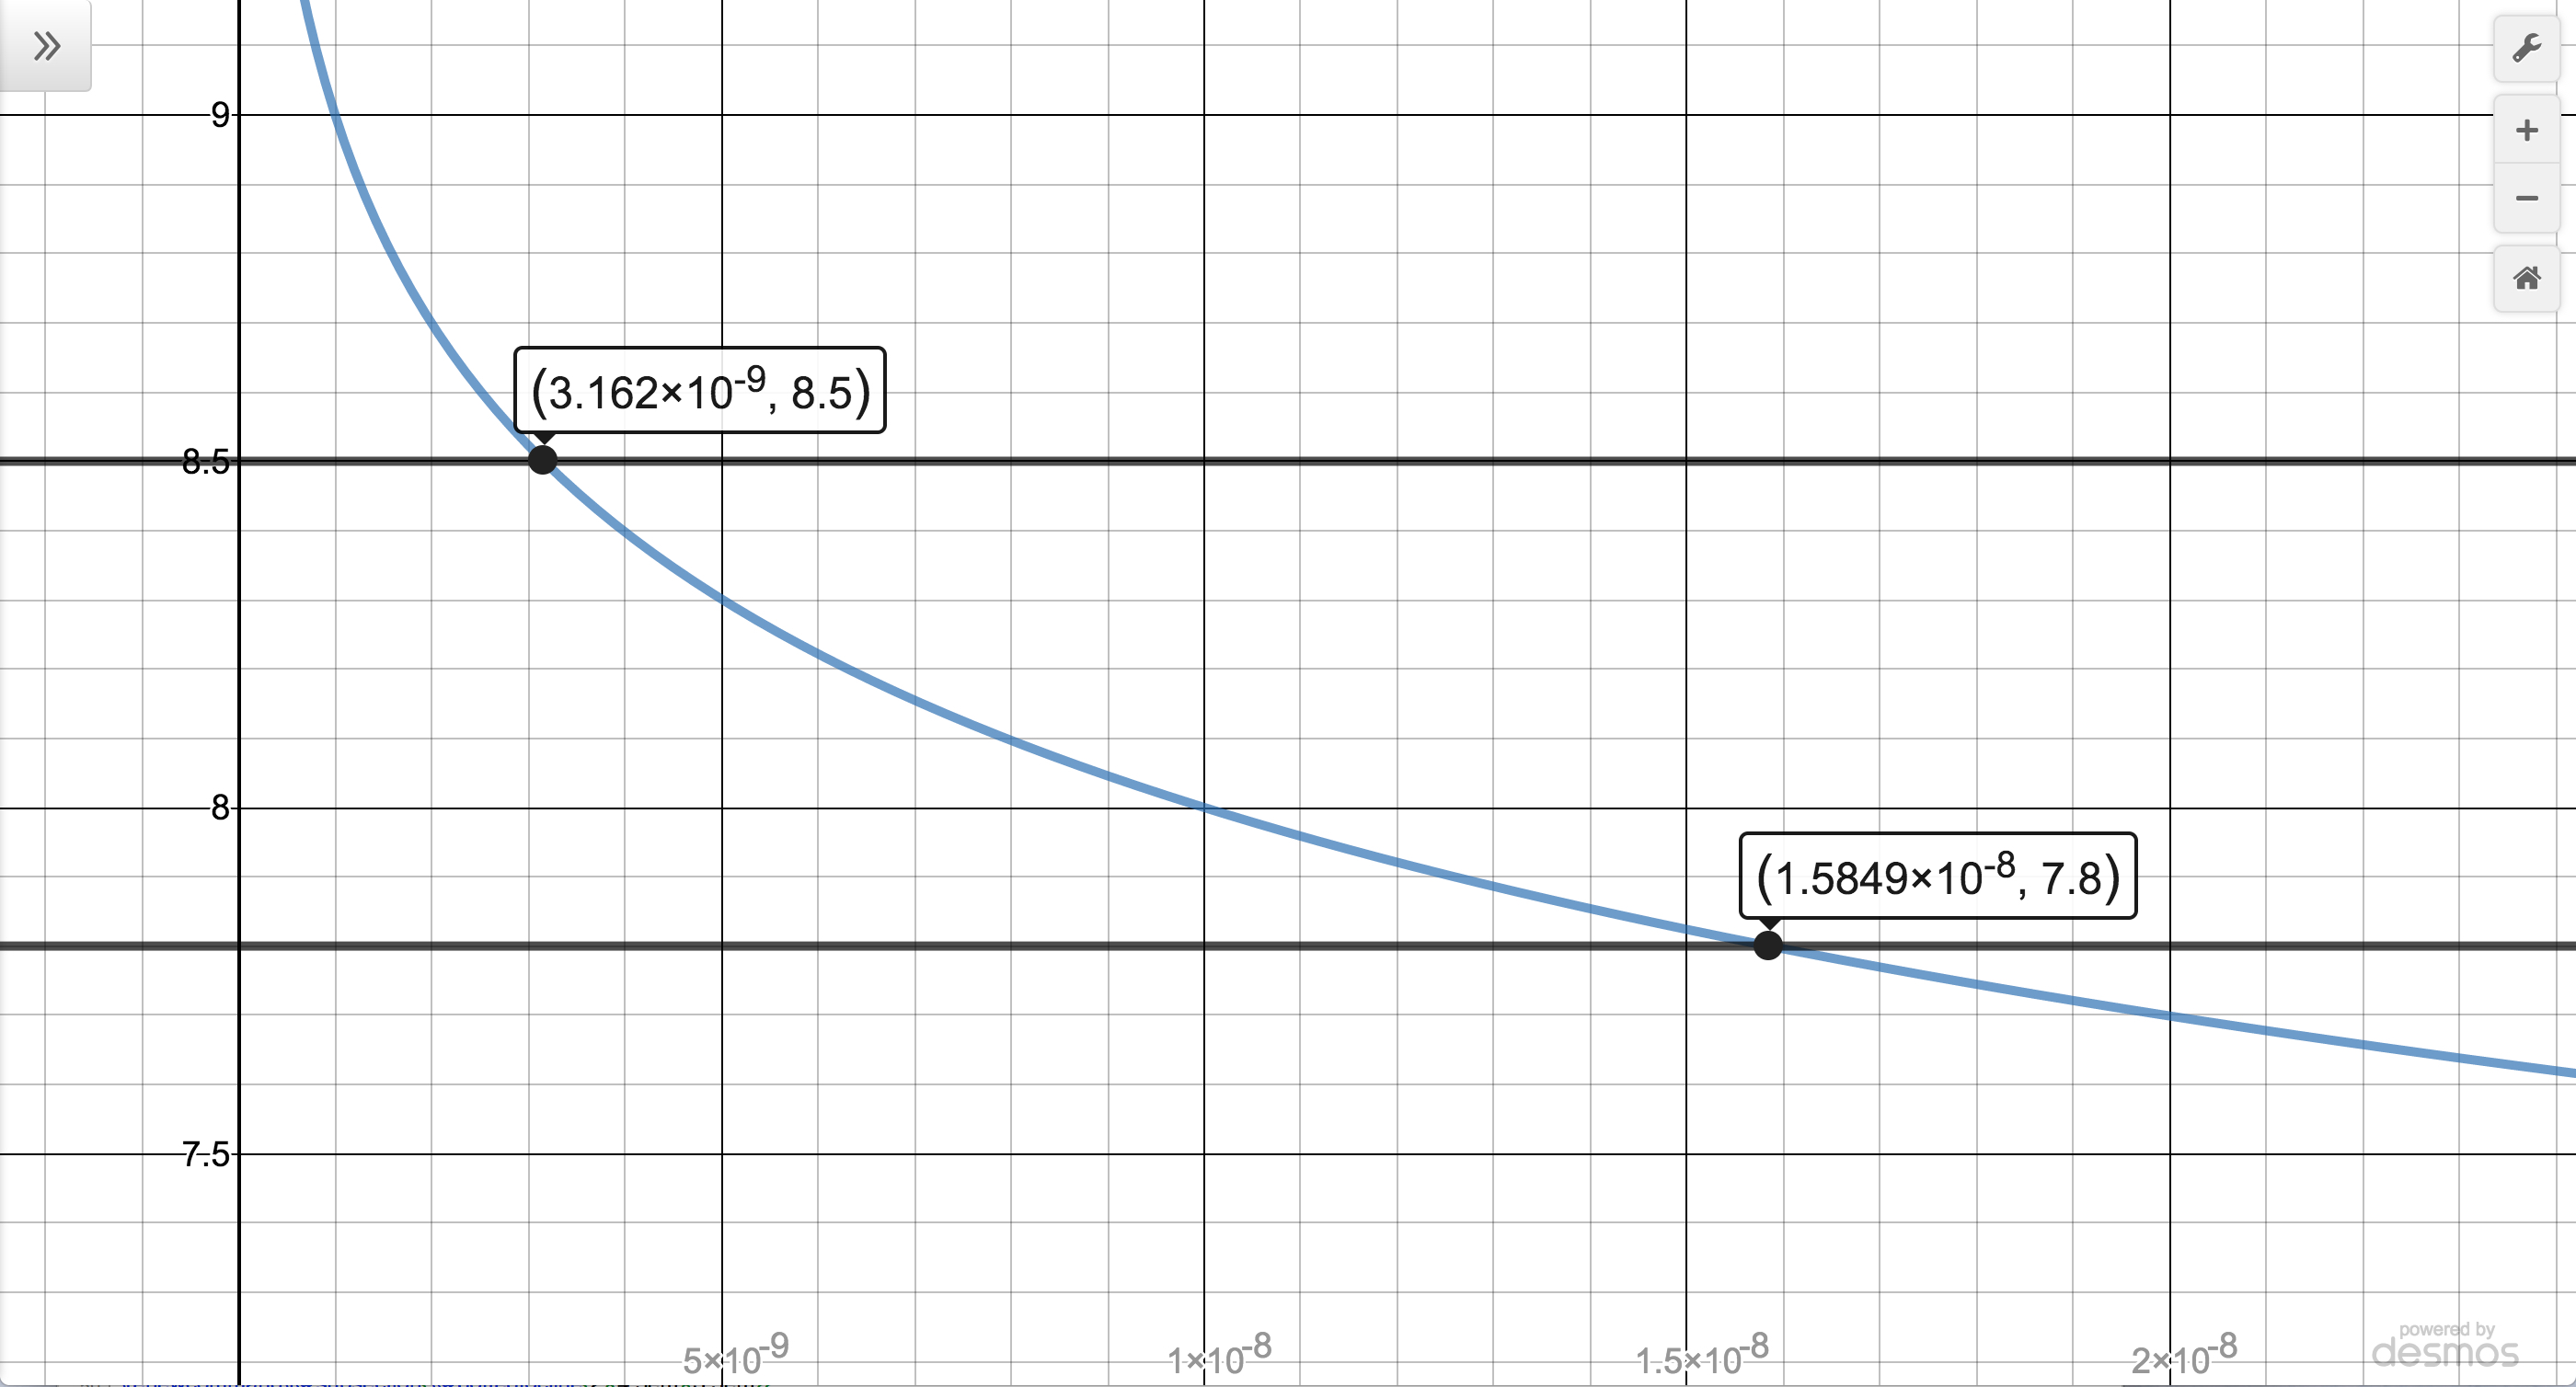
\includegraphics[width=4in]{./LogarithmicEquationsandInequalitiesGraphics/LogEqnEx10.jpg}

\end{center}

\qed

\end{example}

\smallskip

We close this section by finding an inverse of a one-to-one function which involves logarithms.

\begin{example}  \label{logfracinverse} The function $f(x) = \dfrac{\log(x)}{1-\log(x)}$ is one-to-one. 

\begin{enumerate}

\item  Find a formula for $f^{-1}(x)$ and check your answer graphically using a graphing utility.

\item Solve  $\dfrac{\log(x)}{1-\log(x)} = 1$

\end{enumerate}

{\bf Solution.} \begin{enumerate} \item  We first write $y=f(x)$ then interchange the $x$ and $y$ and solve for $y$.

\[ \begin{array}{rclr}
y & = & f(x) & \\ 
y  & = & \dfrac{\log(x)}{1-\log(x)} & \\[8pt]
x  & = & \dfrac{\log(y)}{1-\log(y)} & \text{Interchange $x$ and $y$.}\\[8pt]
x\left(1-\log(y)\right) & = & \log(y) & \\ 
x - x\log(y)  & = & \log(y) & \\ 
x & = & x \log(y) + \log(y) & \\ 
x & = & (x+1) \log(y) & \\ 
\dfrac{x}{x+1}  & = & \log(y) & \\ 
y & = & 10^{\frac{x}{x+1}} & \text{Rewrite as an exponential equation.}\\

\end{array}\]



We have $f^{-1}(x) = 10^{\frac{x}{x+1}}$.  Graphing $f$ and $f^{-1}$ on the same viewing window produces the required symmetry about $y=x$.

\begin{center}

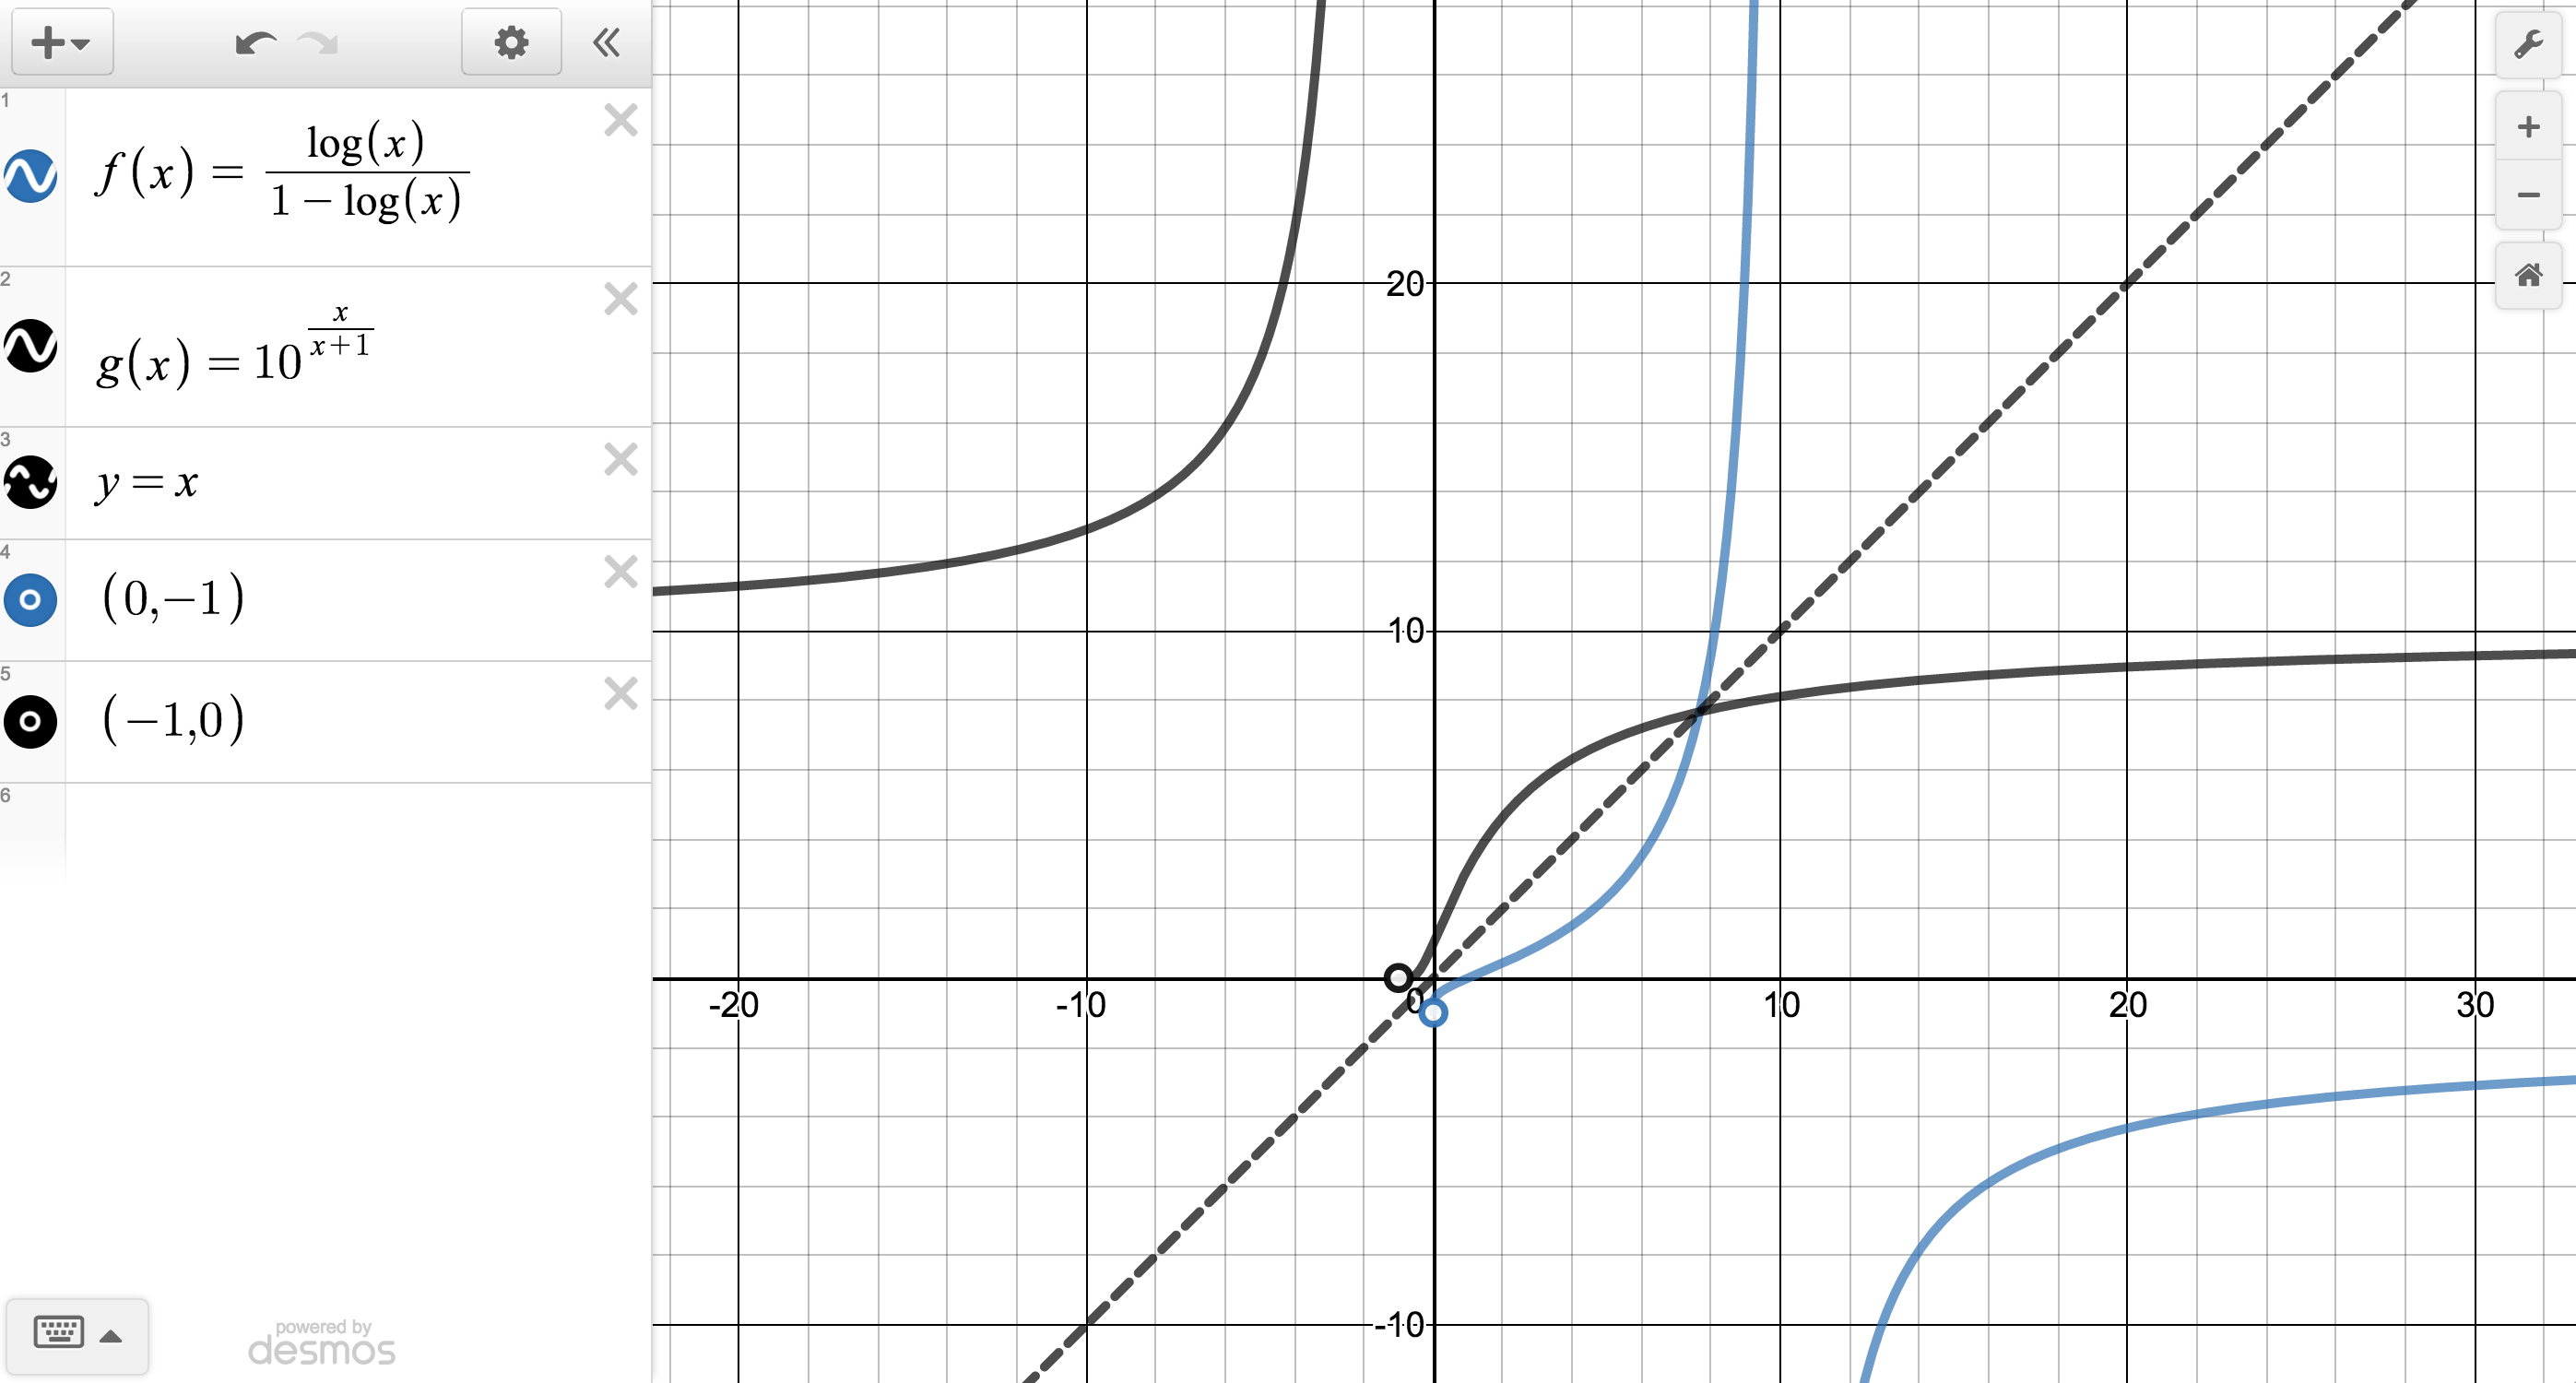
\includegraphics[width=4in]{./LogarithmicEquationsandInequalitiesGraphics/LogEqnEx11.jpg}

\end{center}

\item Recognizing   $\frac{\log(x)}{1-\log(x)} = 1$ as $f(x) = 1$, we have $x = f^{-1}(1) = 10^{\frac{1}{1+1}} = 10^{\frac{1}{2}} = \sqrt{10}$.

To check our answer algebraically,  first recall  $\log(\sqrt{10}) = \log_{10}(\sqrt{10})$.  Next, we know $\sqrt{10} = 10^{\frac{1}{2}}$.  Hence, $\log_{10} \left(10^{\frac{1}{2}} \right) = \frac{1}{2} = 0.5$.  It follows that $\frac{\log(\sqrt{10})}{1-\log(\sqrt{10})} = \frac{0.5}{1-0.5} = \frac{0.5}{0.5} = 1$, as required.  \qed

\end{enumerate}

\end{example}

\pagebreak

Our last example uses the tools from this section along with Section \ref{AppDerivatives}.

\begin{example}\label{logcurvesketchex} Let  $f(x) = x^2 \ln(x)$.

\begin{enumerate}

\item  Find the domain of $f$.

\item  Find the $x$-intercepts, if any.

\item Explain why $\ds{ \lim_{x \rightarrow 0^{+}} x^2 \ln(x)}$ results in an indeterminate form.

Use a table of values  to approximate $\ds{ \lim_{x \rightarrow 0^{+}} x^2 \ln(x)}$.  What does your answer mean graophically? 

\item  Find  $\ds{ \lim_{x \rightarrow \infty} x^2 \ln(x)}$ 

\item  Given $f'(x) = 2x \ln(x) + x$, find the open intervals over which $f$ is increasing and decreasing.

\item  Find the local extrema.

\item  Given $f''(x) = 2 \ln(x) + 3$, find the open intervals over which the graph of $f$ is concave up or concave down.

\item Find the inflection points.

\item  Check your answers using a graphing utility.

\end{enumerate} 

{\bf Solution.}  

\begin{enumerate}

\item  Owing to the presence of the `$\ln(x)$' factor, we have the domain of $f$ is $(0, \infty)$.

\item  To find the $x$-intercepts, we set $f(x) = x^2 \ln(x) = 0$.  This gives $x^2 = 0$ or $\ln(x) = 0$, so $x = 0$ or $x = 1$.  Since $x=0$ is not in the domain of $f$, our only solution is $x = 1$. We have just one $x$-intercept, $(1,0)$.

\item   To analyze $\ds{ \lim_{x \rightarrow 0^{+}} x^2 \ln(x)}$, we note that as $x \rightarrow 0^{+}$, $x^2 \rightarrow 0$ but $\ln(x) \rightarrow -\infty$.  Hence we obtain the indeterminate form\footnote{See the remarks following Example \ref{exponentialcurvesketchingex}.} `$0 \cdot (- \infty)$.'   Making a table of values of $f(x)$ as $x \rightarrow 0^{+}$ suggests  $\ds{ \lim_{x \rightarrow 0^{+}} x^2 \ln(x) = 0}$.  Since $x = 0$ is not in the domain of $f$, there is a hole in the graph at $(0,0)$.

\begin{center}

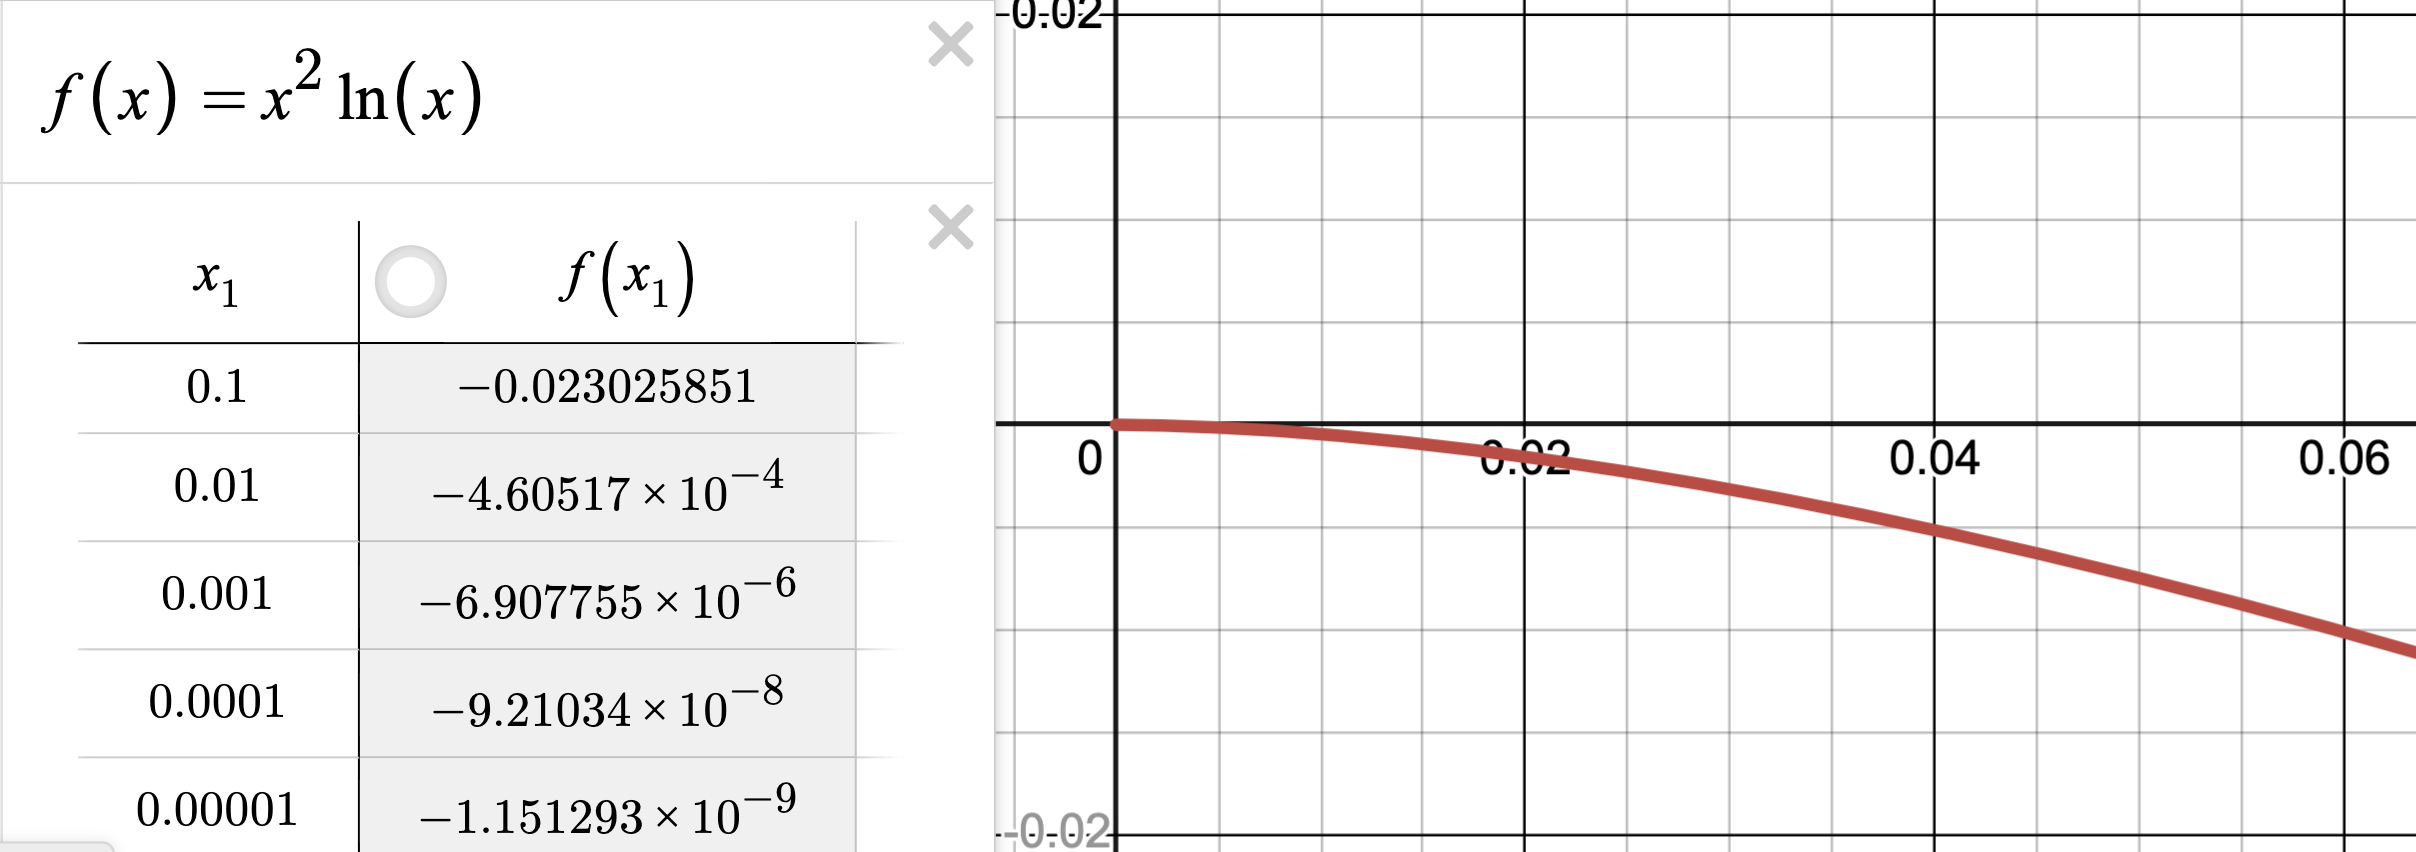
\includegraphics[width=4.5in]{./LogarithmicEquationsandInequalitiesGraphics/x^2ln(x)near0.png}

\end{center}

\item  To determine the intervals over which $f$ is increasing and decreasing, we make a sign diagram for $f'(x) = 2x \ln(x) + x$.  Solving $f'(x) = 2x \ln(x) + x = 0$ we factor: $x(2\ln(x) + 1) = 0$.  Since the domain of $f$ is $(0,
\infty)$, we focus on the factor $2\ln(x) + 1 = 0$.  We get $\ln(x) = -\frac{1}{2}$ so $x = e^{-\frac{1}{2}}$.  

\medskip

When choosing test values, we could opt to find a decimal approximation for $e^{-\frac{1}{2}}$ or we could use more `log-friendly' values.  In this case we note that $e^{-1} < e^{-\frac{1}{2}} < e^{0} = 1$ so we choose $e^{-1}$ and $1$ as our test values.

\medskip

We find $f'\left(e^{-1}\right) = 2 \ln\left(e^{-1}\right) + 1 = 2(-1) + 1 = -1 <0$ and $f'(1) = 2 \ln(1) + 1 = 1 > 0$.  We fill out our sign diagram and interpret accordingly.


\begin{center}

\begin{multicols}{2}

\begin{mfpic}[10]{-6}{6}{-2}{2}
\arrow \polyline{(-6,0),(5,0)}
\xmarks{-6,0}
\arrow \polyline{(-3,-1.5),(-3,-0.5)}
\arrow \polyline{(3,-1.5),(3,-0.5)}
\tlpointsep{4pt}
\axislabels {x}{{$0$} -6, {$e^{-\frac{1}{2}}$} 0}
\tlabel[cc](-3,1){$(-)$}
\tlabel[cc](0,1){$0$}
\tlabel[cc](3,1){$(+)$}
\tlabel[cc](-3,-2.25){$e^{-1}$}
\tlabel[cc](3,-2.25){$1$}
\tlabel[cc](6,1){$f'(x)$}
\tlabel[cc](6,-1){$x$}
%\tlabel[cc](6,0){$\infty$}
%\tlabel[cc](-6,0){$-\infty$}
\end{mfpic}

\begin{mfpic}[10]{-6}{6}{-2}{2}
\arrow  \polyline{(-6,0),(5,0)}
\xmarks{-6, 0}
%\arrow \polyline{(-2,-1.5),(-2,-0.5)}
%\arrow \polyline{(2,-1.5),(2,-0.5)}
\tlpointsep{4pt}
\axislabels {x}{{$0$} -6, {$e^{-\frac{1}{2}}$} 0}
\tlabel[cc](-3,1){$\searrow$}
\tlabel[cc](0,1){$\rightarrow$}
\tlabel[cc](3,1){$\nearrow$}
%\tlabel[cc](-2,-2.25){$0$}
%\tlabel[cc](2,-2.25){$2$}
\tlabel[cc](6,1){$f(x)$}
\tlabel[cc](6,-1){$x$}
%\tlabel[cc](6,0){$\infty$}
%\tlabel[cc](-6,0){$-\infty$}
\end{mfpic}


\end{multicols}
\end{center}

We find $f$ is decreasing on $\left(0, e^{-\frac{1}{2}} \right)$ and increasing on $\left( e^{-\frac{1}{2}}, \infty\right)$.

\item  We see $f$ has a local (and in this case, global) minimum when $x = e^{-\frac{1}{2}}$.  The minimum value is $f\left(e^{-\frac{1}{2}}\right) = \left(e^{-\frac{1}{2}}\right)^2 \ln\left(e^{-\frac{1}{2}}\right) = e^{-1} \left(-\frac{1}{2}\right) = -\frac{e^{-1}}{2}$. The local minimum is $\left( e^{-\frac{1}{2}}, -\frac{e^{-1}}{2} \right)$.



\item  To find the intervals over which the graph of $f$ is concave up and concave down, we make a sign diagram for $f''(x) = 2\ln(x) + 3$.  Solving $f''(x) = 2 \ln(x) + 3 = 0$ we get $\ln(x) = -\frac{3}{2}$ so $x = e^{-\frac{3}{2}}$.  As with our first derivative analysis, we elect to choose some `log-friendly' test values and note $e^{-2} < e^{-\frac{3}{2}} < e^{0} = 1$.  

\medskip

We find $f''\left(e^{-2}\right) = 2 \ln \left(e^{-2}\right) + 3 = 2(-2) + 3 = -1 < 0$ and $f''(1) = 2 \ln(1) + 3 = 3 > 0$.
  
\begin{center}

\begin{multicols}{2}

\begin{mfpic}[10]{-6}{6}{-2}{2}
 \arrow \polyline{(-6,0),(5,0)}
\xmarks{-6,0}
\arrow \polyline{(-3,-1.5),(-3,-0.5)}
\arrow \polyline{(3,-1.5),(3,-0.5)}
\tlpointsep{4pt}
\axislabels {x}{{$0$} -6, {$e^{-\frac{3}{2}}$} 0}
\tlabel[cc](-3,1){$(-)$}
\tlabel[cc](0,1){$0$}
\tlabel[cc](3,1){$(+)$}
\tlabel[cc](-3,-2.25){$e^{-2}$}
\tlabel[cc](3,-2.25){$1$}
\tlabel[cc](6,1){$f''(x)$}
\tlabel[cc](6,-1){$x$}
%\tlabel[cc](6,0){$\infty$}
%\tlabel[cc](-6,0){$-\infty$}
\end{mfpic}

\begin{mfpic}[10]{-6}{6}{-2}{2}
 \arrow \polyline{(-6,0),(5,0)}
\xmarks{-6, 0}
%\arrow \polyline{(-2,-1.5),(-2,-0.5)}
%\arrow \polyline{(2,-1.5),(2,-0.5)}
\tlpointsep{4pt}
\axislabels {x}{{$0$} -6, {$e^{-\frac{3}{2}}$} 0}
\tlabel[cc](-3,1){\Huge $\frown$}
%\tlabel[cc](0,1){$\rightarrow$}
\tlabel[cc](3,1){\Huge $\smile$}
%\tlabel[cc](-2,-2.25){$0$}
%\tlabel[cc](2,-2.25){$2$}
\tlabel[cc](6,1){$f(x)$}
\tlabel[cc](6,-1){$x$}
%\tlabel[cc](6,0){$\infty$}
%\tlabel[cc](-6,0){$-\infty$}
\end{mfpic}


\end{multicols}
\end{center}

We see the graph of $f$ is concave down on $\left(0, e^{-\frac{3}{2}} \right)$ and concave up on $\left(e^{-\frac{3}{2}} , \infty \right)$.


\item  Since the concavity changes at $x = e^{-\frac{3}{2}}$, we have an inflection point at $\left( e^{-\frac{3}{2}}, f \left(e^{-\frac{3}{2}}\right) \right)$.  We find $f \left(e^{-\frac{3}{2}}\right)  = \left(f \left(e^{-\frac{3}{2}}\right) \right)^2 \ln \left(f \left(e^{-\frac{3}{2}}\right) \right) = e^{-3} \left(-\frac{3}{2} \right) = -\frac{3e^{-3}}{2}$.  Our inflection point is $\left( e^{-\frac{3}{2}},  -\frac{3e^{-3}}{2} \right)$.

\item  Using  \href{https://www.desmos.com/calculator}{\underline{desmos}}, we confirm our calculations.\footnote{It may require some window adjustment to capture the inflection point.}

\begin{center}

\begin{multicols}{2}

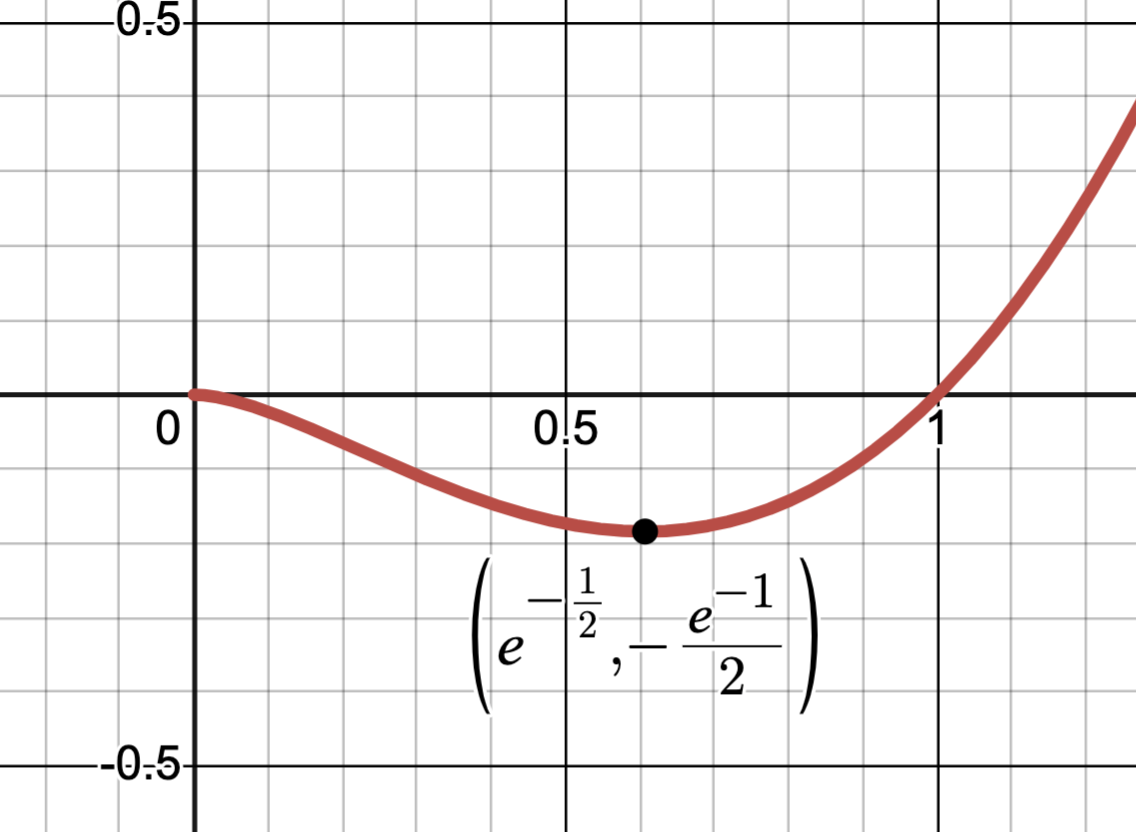
\includegraphics[width=2.5in]{./LogarithmicEquationsandInequalitiesGraphics/x^2ln(x)min.png}

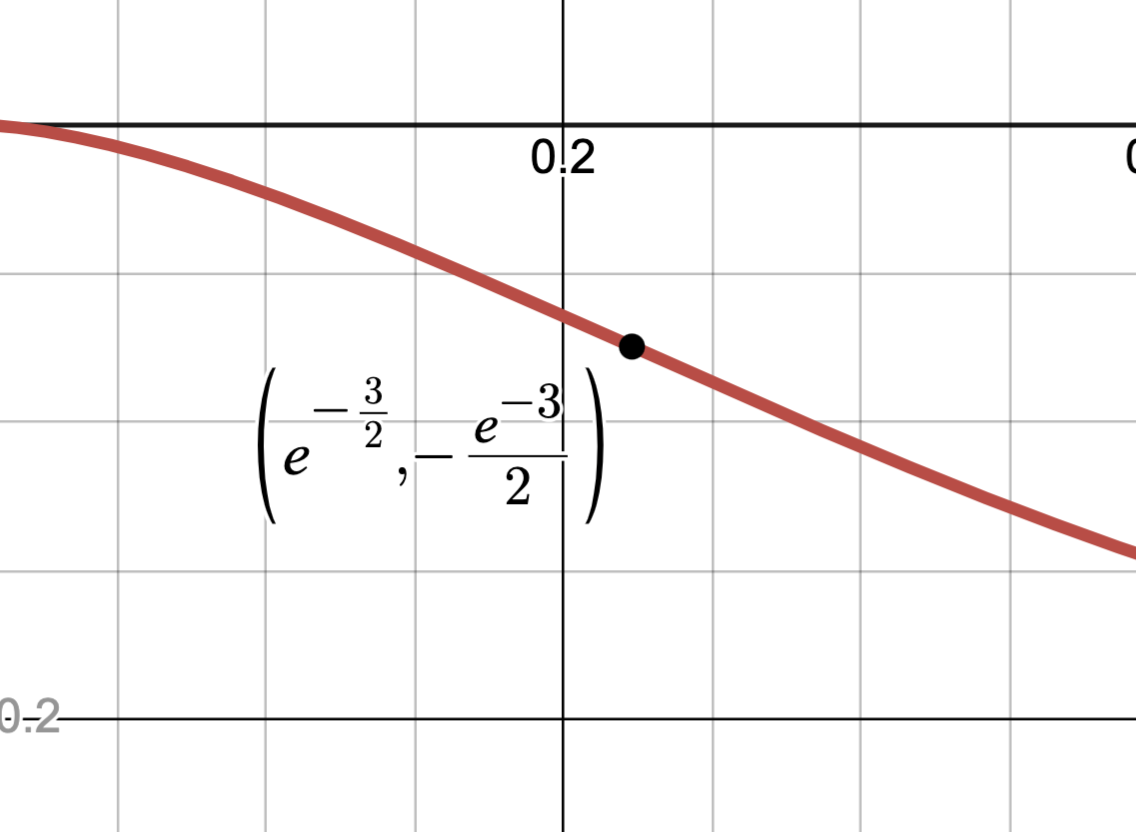
\includegraphics[width=2.5in]{./LogarithmicEquationsandInequalitiesGraphics/x^2ln(x)IP.png} \\

\end{multicols}

\end{center}

\hfill \qed

\end{enumerate}

\end{example}

When determining $\ds{\lim_{x \rightarrow 0^{+}} f(x)  = \lim_{x \rightarrow 0^{+}} x^2 \ln(x) }$ in Example \ref{logcurvesketchex}, we encountered the indeterminate form `$0 \cdot (-\infty)$.'  This is a similar scenario to what we encountered in the remarks following Example \ref{exponentialcurvesketchingex} in Section \ref{ExponentialEquationsandInequalities}.  I this case, the factor $x^2 \rightarrow 0$ and the factor $\ln(x) \rightarrow -\infty$ and so we have a tug-of-war to see which factor's behavior will win out over the other.  Here, $x^2 \rightarrow 0$ dominates as the table suggests $\ds{\lim_{x \rightarrow 0^{+}} x^2 \ln(x) = 0}$.  This is indeed the case and, in general, polynomials (and, in general, all positive powers of $x$) dominate logarithms as we'll explore in the Exercise \ref{numericalinvestigationlimitlnxtimesx}.  

\newpage

\subsection{Exercises}

%% SKIPPED %% \label{ExercisesforLogarithmicEquationsandInequalities}

In Exercises \ref{solvelogeqexfirst} - \ref{solvelogeqexlast}, solve the equation analytically.

\begin{multicols}{2}
\begin{enumerate}

\item $\log(3x-1) = \log(4-x)$  \phantom{$\log_{2}\left(x^{3}\right) = \log_{2}(x)$} \label{solvelogeqexfirst}

\item $\log_{2}\left(x^{3}\right) = \log_{2}(x)$

\setcounter{HW}{\value{enumi}}
\end{enumerate}
\end{multicols}

\begin{multicols}{2}
\begin{enumerate}
\setcounter{enumi}{\value{HW}}

\item $\ln\left(8-t^2\right)=\ln(2-t)$ \vphantom{$\log_{5}\left(18-t^2\right) = \log_{5}(6-t)$}

\item $\log_{5}\left(18-t^2\right) = \log_{5}(6-t)$

\setcounter{HW}{\value{enumi}}
\end{enumerate}
\end{multicols}

\begin{multicols}{2}
\begin{enumerate}
\setcounter{enumi}{\value{HW}}

\item $\log_{3}(7-2x) = 2$ \vphantom{$\log_{\frac{1}{2}} (2x-1) = -3$}
\item $\log_{\frac{1}{2}} (2x-1) = -3$

\setcounter{HW}{\value{enumi}}
\end{enumerate}
\end{multicols}

\begin{multicols}{2}
\begin{enumerate}
\setcounter{enumi}{\value{HW}}

\item $\ln\left(t^2-99\right) = 0$
\item $\log(t^2-3t) = 1$

\setcounter{HW}{\value{enumi}}
\end{enumerate}
\end{multicols}

\begin{multicols}{2}
\begin{enumerate}
\setcounter{enumi}{\value{HW}}

\item $\log_{125} \left(\dfrac{3x-2}{2x+3}\right)=\dfrac{1}{3}$

\item $\log\left(\dfrac{x}{10^{-3}}\right) = 4.7$ \vphantom{$\log_{125} \left(\dfrac{3x-2}{2x+3}\right)$} \label{sixfourRichterequ}


\setcounter{HW}{\value{enumi}}
\end{enumerate}
\end{multicols}


\begin{multicols}{2}
\begin{enumerate}
\setcounter{enumi}{\value{HW}}

\item $-\log(x) = 5.4$ \vphantom{$10\log\left(\dfrac{t}{10^{-12}}\right)$} \label{sixfourpHequ}
\item $10\log\left(\dfrac{x}{10^{-12}}\right) = 150$ \label{sixfourdecibelequ}

\setcounter{HW}{\value{enumi}}
\end{enumerate}
\end{multicols}

\begin{multicols}{2}
\begin{enumerate}
\setcounter{enumi}{\value{HW}}

\item $6-3\log_{5}(2t)=0$
\item $3\ln(t)-2=1-\ln(t)$

\setcounter{HW}{\value{enumi}}
\end{enumerate}
\end{multicols}

\begin{multicols}{2}
\begin{enumerate}
\setcounter{enumi}{\value{HW}}

\item $\log_{3}(t - 4) + \log_{3}(t + 4) = 2$

\item $\log_{5}(2t + 1) + \log_{5}(t + 2) = 1$

\setcounter{HW}{\value{enumi}}
\end{enumerate}
\end{multicols}

\begin{multicols}{2}
\begin{enumerate}
\setcounter{enumi}{\value{HW}}

\item $\log_{169}(3x + 7) - \log_{169}(5x - 9) = \dfrac{1}{2}$

\item $\ln(x+1) - \ln(x) = 3$ \vphantom{$\log_{169}(3x + 7)$}

\setcounter{HW}{\value{enumi}}
\end{enumerate}
\end{multicols}

\begin{multicols}{2}
\begin{enumerate}
\setcounter{enumi}{\value{HW}}

\item $2\log_{7}(t) = \log_{7}(2) + \log_{7}(t+12)$

\item $\log(t) - \log(2) = \log(t+8)  - \log(t+2)$

\setcounter{HW}{\value{enumi}}
\end{enumerate}
\end{multicols}

\begin{multicols}{2}
\begin{enumerate}
\setcounter{enumi}{\value{HW}}

\item $\log_{3}(x) = \log_{\frac{1}{3}}(x) + 8$

\item $\ln(\ln(x)) = 3$

\setcounter{HW}{\value{enumi}}
\end{enumerate}
\end{multicols}

\begin{multicols}{2}
\begin{enumerate}
\setcounter{enumi}{\value{HW}}

\item $\left(\log(t)\right)^2=2\log(t)+15$

\item $\ln(t^{2}) = (\ln(t))^{2}$ \label{solvelogeqexlast}

\setcounter{HW}{\value{enumi}}
\end{enumerate}
\end{multicols}


In Exercises \ref{solvelogineqexfirst} - \ref{solvelogineqexlast}, solve the inequality analytically.

\begin{multicols}{2}
\begin{enumerate}
\setcounter{enumi}{\value{HW}}

\item $\dfrac{1 - \ln(t)}{t^{2}} < 0$ \label{solvelogineqexfirst}
\item $t\ln(t) - t > 0$ \phantom{$\dfrac{1 - \ln(x)}{x^{2}} < 0$}  


\setcounter{HW}{\value{enumi}}
\end{enumerate}
\end{multicols}

\begin{multicols}{2}
\begin{enumerate}
\setcounter{enumi}{\value{HW}}

\item $10\log\left(\dfrac{x}{10^{-12}}\right) \geq 90$ \label{sixfourdecibelineq} 
\item $5.6 \leq \log\left(\dfrac{x}{10^{-3}}\right) \leq 7.1$ \label{sixfourRichterineq}


\setcounter{HW}{\value{enumi}}
\end{enumerate}
\end{multicols}

\begin{multicols}{2}
\begin{enumerate}
\setcounter{enumi}{\value{HW}}


\item $2.3 < -\log(x) < 5.4$ \label{sixfourpHineq} 

\item $\ln(t^{2}) \leq (\ln(t))^{2}$ \label{solvelogineqexlast} 

\setcounter{HW}{\value{enumi}}
\end{enumerate}
\end{multicols}

\pagebreak

In Exercises \ref{logeqcalcexfirst} - \ref{logeqcalcexlast}, use a graphing utility to help you solve the equation or  inequality.

\begin{multicols}{2}
\begin{enumerate}
\setcounter{enumi}{\value{HW}}

\item $\ln(t) = e^{-t}$ \label{logeqcalcexfirst} 
\item $\ln(x) = \sqrt[4]{x}$ 

\setcounter{HW}{\value{enumi}}
\end{enumerate}
\end{multicols}

\begin{multicols}{2}
\begin{enumerate}
\setcounter{enumi}{\value{HW}}

\item $\ln(t^{2} + 1) \geq 5$
\item $\ln(-2x^{3} - x^{2} + 13x - 6) < 0$ \label{logeqcalcexlast} 

\setcounter{HW}{\value{enumi}}
\end{enumerate}
\end{multicols}


In Exercises \ref{domaincomplicatedlogfirst} - \ref{domaincomplicatedloglast},  find the domain of the function.

\begin{multicols}{2} 
\begin{enumerate}
\setcounter{enumi}{\value{HW}}

\item \label{domaincomplicatedlogfirst}  $r(x) =   \dfrac{x}{1 - \ln(x)}$  %(-\infty, e) \cup (e, \infty)$

\item   $R(x) = \dfrac{x \ln(x)}{1 - \ln(x)}$   % $(0,e) \cup (e, \infty)$

\setcounter{HW}{\value{enumi}}
\end{enumerate}
\end{multicols}


\begin{multicols}{2} 
\begin{enumerate}
\setcounter{enumi}{\value{HW}}

\item     $s(t) = \sqrt{2 - \log(t)}$  \vphantom{$c(t) =  (2 \ln(t) -1)^{\frac{2}{3}}$} %$(0, 100]$
\item     $c(t) =  (2 \ln(t) -1)^{\frac{2}{3}}$  %$(0, \infty)$

\setcounter{HW}{\value{enumi}}
\end{enumerate}
\end{multicols}

\begin{multicols}{2} 
\begin{enumerate}
\setcounter{enumi}{\value{HW}}
  
\item     $\ell(t) = \ln( \ln(t))$  \vphantom{$L(x) = \log\left( \dfrac{x \ln(x)}{1 - \ln(x)} \right)$} %$(1, \infty)$    

\item  \label{domaincomplicatedloglast}    $L(x) = \log\left( \dfrac{x \ln(x)}{1 - \ln(x)} \right)$  %$(1,e)$ 


\setcounter{HW}{\value{enumi}}
\end{enumerate}
\end{multicols}


\begin{enumerate}
\setcounter{enumi}{\value{HW}}

\item \label{onetooneexpexercise} Since $f(x) = e^{x}$ is a strictly increasing function, if $a < b$ then $e^{a} < e^{b}$.  Use this fact to solve the inequality $\ln(2x + 1) < 3$ without a sign diagram. Use this technique to solve the inequalities in Exercises \ref{sixfourdecibelineq} - \ref{sixfourpHineq}. (Compare this to Exercise  \ref{onetoonelogexercise} in Section \ref{ExponentialEquationsandInequalities}.)

\item Solve $\ln(3 - y) - \ln(y) = 2x + \ln(5)$ for $y$.

\item In Example \ref{logfracinverse} we found the inverse of $f(x) = \dfrac{\log(x)}{1-\log(x)}$ to be $f^{-1}(x) = 10^{\frac{x}{x+1}}$.

\begin{enumerate}

\item Algebraically check our answer by verifying  $\left(f^{-1} \circ f\right)(x) = x$ for all $x$ in the domain of $f$ and that $\left(f \circ f^{-1}\right)(x) = x$ for all $x$ in the domain of $f^{-1}$.

\item Find the range of $f$ by finding the domain of $f^{-1}$.

\item Let $g(x) = \dfrac{x}{1 - x}$ and $h(x) = \log(x)$.  Show that $f = g \circ h$ and $(g \circ h)^{-1} = h^{-1} \circ g^{-1}$.\\


NOTE:  We know this is true in general by Exercise \ref{fcircginverse} in Section \ref{InverseFunctions}, but it's nice to see a specific example of the property.

\end{enumerate}

\item \label{inversehyptangent} Let $f(x) = \dfrac{1}{2}\ln\left(\dfrac{1 + x}{1 - x}\right)$.  Compute $f^{-1}(x)$ and find its domain and range.

\item Explain the equation in Exercise \ref{sixfourRichterequ} and the inequality in Exercise \ref{sixfourRichterineq} above in terms of the Richter scale for earthquake magnitude.  (See Exercise \ref{Richterexercise} in Section \ref{ExponentialFunctions}.)

\item Explain the equation in Exercise \ref{sixfourdecibelequ} and the inequality in Exercise \ref{sixfourdecibelineq} above in terms of sound intensity level as measured in decibels.  (See Exercise \ref{decibelexercise} in Section \ref{ExponentialFunctions}.)

\item Explain the equation in Exercise \ref{sixfourpHequ} and the inequality in Exercise \ref{sixfourpHineq} above in terms of the pH of a solution.  (See Exercise \ref{pHexercise} in Section \ref{ExponentialFunctions}.)

\item With the help of your classmates, solve the inequality $\sqrt[n]{x} > \ln(x)$ for a variety of natural numbers $n$.  What might you conjecture about the ``speed'' at which $f(x) = \ln(x)$ grows versus any principal $n^{\textrm{th}}$ root function?

\end{enumerate}

\newpage

\subsection{Answers}
\begin{multicols}{3}
\begin{enumerate}

\item $x = \frac{5}{4}$
\item $x = 1$
\item $t=-2$

\setcounter{HW}{\value{enumi}}
\end{enumerate}
\end{multicols}

\begin{multicols}{3}
\begin{enumerate}
\setcounter{enumi}{\value{HW}}

\item $t=-3,\, 4$
\item $x=-1$
\item $x=\frac{9}{2}$

\setcounter{HW}{\value{enumi}}
\end{enumerate}
\end{multicols}

\begin{multicols}{3}
\begin{enumerate}
\setcounter{enumi}{\value{HW}}

\item $t=\pm 10$
\item $t=-2,\, 5$
\item $x = -\frac{17}{7}$

\setcounter{HW}{\value{enumi}}
\end{enumerate}
\end{multicols}

\begin{multicols}{3}
\begin{enumerate}
\setcounter{enumi}{\value{HW}}

\item $x = 10^{1.7}$
\item $x = 10^{-5.4}$
\item $x = 10^{3}$

\setcounter{HW}{\value{enumi}}
\end{enumerate}
\end{multicols}

\begin{multicols}{3}
\begin{enumerate}
\setcounter{enumi}{\value{HW}}

\item $t=\frac{25}{2}$
\item $t=e^{3/4}$
\item $t = 5$

\setcounter{HW}{\value{enumi}}
\end{enumerate}
\end{multicols}

\begin{multicols}{3}
\begin{enumerate}
\setcounter{enumi}{\value{HW}}

\item $t = \frac{1}{2}$
\item $x = 2$
\item $x = \frac{1}{e^3-1}$

\setcounter{HW}{\value{enumi}}
\end{enumerate}
\end{multicols}

\begin{multicols}{3}
\begin{enumerate}
\setcounter{enumi}{\value{HW}}

\item $t=6$
\item $t=4$
\item $x = 81$

\setcounter{HW}{\value{enumi}}
\end{enumerate}
\end{multicols}

\begin{multicols}{3}
\begin{enumerate}
\setcounter{enumi}{\value{HW}}

\item $x = e^{e^3}$
\item $t=10^{-3}, \, 10^{5}$
\item $t = 1, \, x = e^{2}$

\setcounter{HW}{\value{enumi}}
\end{enumerate}
\end{multicols}

\begin{multicols}{3}
\begin{enumerate}
\setcounter{enumi}{\value{HW}}

\item $(e, \infty)$
\item $(e, \infty)$
\item $\left[10^{-3}, \infty \right)$

\setcounter{HW}{\value{enumi}}
\end{enumerate}
\end{multicols}

\begin{multicols}{3}
\begin{enumerate}
\setcounter{enumi}{\value{HW}}

\item $\left[10^{2.6}, 10^{4.1}\right]$

\item $\left(10^{-5.4}, 10^{-2.3}\right)$
\item $(0, 1] \cup [e^{2}, \infty)$

\setcounter{HW}{\value{enumi}}
\end{enumerate}
\end{multicols}

\begin{multicols}{2}
\begin{enumerate}
\setcounter{enumi}{\value{HW}}

\item $t \approx 1.3098$
\item $x \approx 4.177, \, x \approx 5503.665$

\setcounter{HW}{\value{enumi}}
\end{enumerate}
\end{multicols}

\begin{multicols}{2}
\begin{enumerate}
\setcounter{enumi}{\value{HW}}

\item $\approx (-\infty, -12.1414) \cup (12.1414, \infty)$
\item $\approx (-3.0281, -3) \cup (0.5, 0.5991) \cup (1.9299, 2)$

\setcounter{HW}{\value{enumi}}
\end{enumerate}
\end{multicols}

\begin{multicols}{3} 
\begin{enumerate}
\setcounter{enumi}{\value{HW}}

\item  $(-\infty, e) \cup (e, \infty)$

\item   $(0,e) \cup (e, \infty)$

\item  $(0, 100]$

\setcounter{HW}{\value{enumi}}
\end{enumerate}
\end{multicols}


\begin{multicols}{3} 
\begin{enumerate}
\setcounter{enumi}{\value{HW}}

\item    $(0, \infty)$
  
\item    $(1, \infty)$    

\item    $(1,e)$ 


\setcounter{HW}{\value{enumi}}
\end{enumerate}
\end{multicols}


\begin{multicols}{2}
\begin{enumerate}
\setcounter{enumi}{\value{HW}}

\item $-\dfrac{1}{2} < x < \dfrac{e^{3} - 1}{2}$, so $\left( -\dfrac{1}{2}, \dfrac{e^{3} - 1}{2}\right)$

\item $y = \dfrac{3}{5e^{2x} + 1}$ \vphantom{$\dfrac{e^{3} - 1}{2}$}

\setcounter{HW}{\value{enumi}}
\end{enumerate}
\end{multicols}

\begin{enumerate}
\setcounter{enumi}{\value{HW}}
\addtocounter{enumi}{1}

\item $f^{-1}(x) = \dfrac{e^{2x} - 1}{e^{2x} + 1} = \dfrac{e^{x} - e^{-x}}{e^{x} + e^{-x}}$. 

To see why we rewrite this in this form, see  Exercise \ref{andtheresthyperbolic} in Section \ref{ParametricEquations}.

 The domain of $f^{-1}$ is $(-\infty, \infty)$ and its range is the same as the domain of $f$, namely $(-1, 1)$.

\end{enumerate}



\closegraphsfile

\end{document}
